% !TeX root = ../../thesis.tex
\chapter{Ambient Stability of Thermally Co-Evaporated \ch{CsPbI_2Br} Thin Films}\label{ch:stability}


So far, thermally co-evaporated \ch{CsPbI_2Br} thin films have enabled the fabrication of vacuum-deposited photodiodes with competitive performance and excellent high-temperature tolerance. However, one critical aspect, which is also one of the inherent limitations of \ch{CsPbI_xBr_{3-x}} (1<x<3) perovskites, remains unaddressed: their phase instability, particularly in the presence of moisture. In this chapter, we explore the factors influencing perovskite phase instability, with a particular emphasis on thermally evaporated thin films. Followingly, we attempt to benchmark the stability of our thermally co-evaporated \ch{CsPbI_2Br} thin films, however challenges in the reproducibility of experimental data motivates us to adopt a combinatorial, high-throughput experimentation approach. The latter allows us to investigate the impact of precursor stoichiometry, substrate type, and perovskite thickness. Building on these insights, we fabricate top-illuminated PePDs and assess their performance over multiple days of exposure to open-air conditions.


\section{Origins of Ambient (In)-Stability}

As discussed in Section~\ref{ch1:scalable_high_temp}, the perovskite compositions \ch{CsPbI_3} and \ch{CsPbI_2Br} exist in two distinct structural forms: the black phase (which includes cubic, tetragonal, and orthorhombic polymorphs) and the yellow phase. For \ch{CsPbI_3}, the thermodynamically favored phase at room temperature is the yellow one, which, due to its significantly larger bandgap ($\sim$2.8 eV), is unsuitable for optoelectronic applications. While it is possible to "trap" the black phase at room temperature under inert conditions (e.g., in a nitrogen environment), it remains prone to conversion \cite{Steele2021TrojansPerovskite}. The yellow phase rapidly re-emerges upon mild heating (around 60\degree C) or exposure to ambient moisture. In the former case, the thermal energy is sufficient to overcome the activation barrier for the phase transition \cite{Steele2019ThermalFilms}. In the latter, water molecules adsorbed on the perovskite surface act as catalysts, promoting the formation of halide vacancies, which, in turn, lowers the free energy barrier between the two phases \cite{Dastidar2016HighIodide, Kang2017HighCsPbBr3, Lin2018ThermochromicCells, Lin2021KineticsPerovskite}. 


The challenges of stabilizing the black perovskite phase at room temperature (in inert environment), as well as the prevention of conversion at mild temperatures are both successfully tackled with the introduction of \ch{Br^-} into the lattice and the formation of the \ch{CsPbI_2Br} composition \cite{Sutton2016Bandgap-TunableCells}. For example, \ch{CsPbI_2Br} thin films can be stored unaltered in a N2 glovebox for months or even years, while the black phase is retained even under continuous heating from room temperature to beyond 300\degree 
C \cite{Papadopoulou2024InEllipsometry}. The enhanced stability is attributed to the smaller ionic radius of \ch{Br^-}, which, in turn, increases the Goldschmidt tolerance factor (Eq.~\ref{eq:tolerance_factor}) of the composition. However, the issue of phase conversion upon exposure to ambient moisture remains unresolved, with reported stabilities ranging from just a few minutes to several days \cite{Zhu2022UnderstandingPerovskites, Zheng2021ImprovedCells, Mariotti2018StabilityDevices}. 

Strategies to improve the ambient stability of \ch{CsPbI_3} and \ch{CsPbI_2Br} have been primarily investigated for solution processed, and more specifically spin-coated, thin films. These techniques can be distinguished into i) \ch{ABX_3} site doping, ii) incorporation of additives into the perovskite solution, iii) surface functionalization, or iv) dimensionality engineering \cite{Jin2024PhaseDevices}. However, due to the fundamentally different deposition conditions and crystal growth involved in thermal co-evaporation, the effectiveness of these strategies might be inherently non-transferable or difficult to replicate in vacuum-deposited perovskite systems. For instance, the approaches of surface functionalization and additive inclusion typically rely on the use of organic components, such as DMAI (dimethylammonium iodide), PEAI (phenethylammonium iodide), \ch{DETAI_3} (diethylenetriamine iodide), which could potentially compromise the thermal stability of our device stack. The strategy of introducing \ch{ABX_3} site doping might seem more easily transferable through the co-evaporation of necessary precursors. For instance, the use of bismuth (Bi) as a B-site dopant has been shown to drastically improve the stability of $\gamma-$\ch{CsPbI_2Br} solution-processed thin films \cite{Hu2017BismuthCells}. However, when Yang et al. attempted to deposit \ch{CsPb_{0.96}Bi_{0.04}I_3} thin films via the co-evaporation of CsI and \ch{Pb_{1-x}Bi_xI_2} powders, they discovered that, when evaporated, the targeted composition is not a thermodynamically favored black phase system, despite its improved tolerance factor \cite{Yang2021CanPhase}.


An additional option for improving the stability of perovskite films, which is not directly linked to the deposition method, is through strain engineering. Multiple avenues for introducing strain in the lattice have been explored. These can include the introduction of surface strain through rapid cooling (taking advantage of the large mismatch between the thermal expansion coefficient of the perovskite and the substrate) or the use of substrates with scaffold-like structure \cite{Steele2019ThermalFilms, Chakrabarti2022Scaffold-EnforcedStability}. The introduction of vertical strain has been demonstrated through the scribing of a \ch{PbI_2} microstructure via laser writing or the growth of the perovskite on top of vertically aligned anodized aluminum oxide nanopores \cite{Steele2022AnFilms, Ma2019Strain-MediatedGrowth}. Even the stability-enhancement approaches described earlier, such as the inclusion of additives or dimensionality engineering, have been partially attributed to an increment of strain in the lattice \cite{Steele2021TrojansPerovskite}. Nevertheless, the introduction of stress into the lattice for the improvement of phase stability does not come without trade-offs. Previous studies revealed that the elimination of tensile strain in the lattice is critical for enhancing the stability of PCE and eliminating phase segregation under continuous illumination \cite{Rolston2018EngineeringStability, Xue2020RegulatingLayers}.

\begin{figure}[htbp]
    \centering
    % Second row
    \begin{subfigure}[t]{0.99\textwidth}
        \centering
        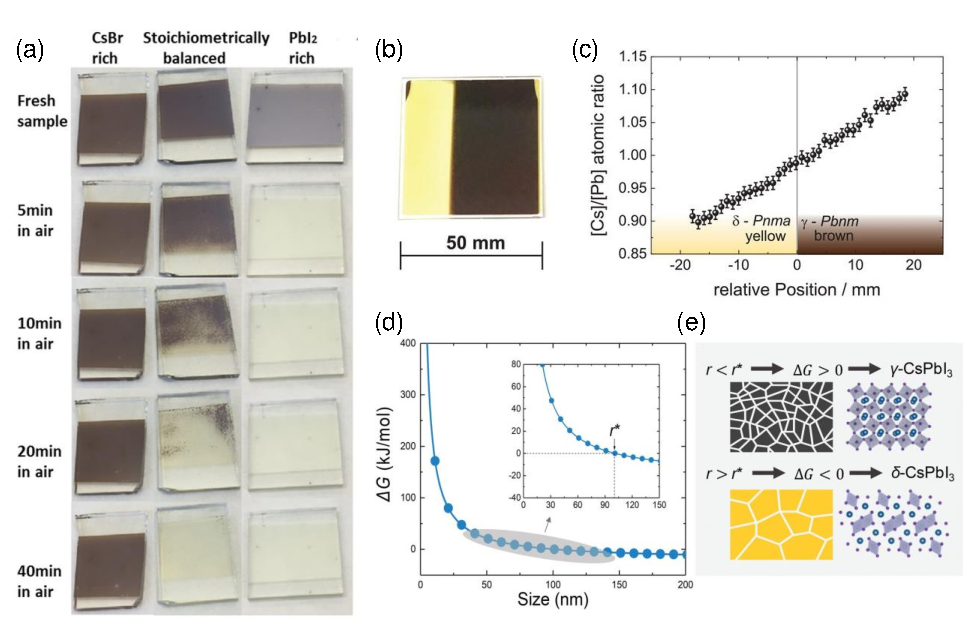
\includegraphics[width=\textwidth]{chapters/stability/imeges/Stability_Lierature.pdf} % Replace with your image file                
    \end{subfigure}

    \caption{Literature review on studies evaluating the phase stability of \ch{CsPbI_3} ans \ch{CsPbI_2Br} thin films. (a) Rate of brown-to-yellow phase conversion for CsBr-rich, stoichiometrically balanced, and \ch{PbI_2}-rich \ch{CsPbI_2Br} thin films. Reproduced from \cite{Ma2017TheCells}. (b) Appearance of phase boundary on an as-deposited \ch{CsPbI_3} thin film deposited via the co-evaporation of CsI and \ch{PbI_2} without substrate rotation. (c) According to XRF measurements, the boundary separates the Cs-rich from the Pb-rich region. Reproduced from \cite{Becker2019LowExperimentation}. (d) Impact of grain size on the Gibbs free energy difference between the $\delta-$ and the $\gamma-$phase ($\Delta G$).  (e) Once the grain size (r) is smaller than a critical value ($r^*$), the $\gamma-$phase is preferred. Reproduced from \cite{Dong2023GrowthFilm}. }
    \label{fig:stability:literature_review}
\end{figure}


The phase and ambient stability of thermally evaporated \ch{CsPbI_3} and \ch{CsPbI_2Br} thin films has been investigated in a limited number of reports, which however can provide crucial insights. For instance, Ma et al. identified that during the co-evaporation of CsBr and \ch{PbI_2} for the deposition of \ch{CsPbI_2Br} thin films, the precursor ratio has a critical impact on the ambient stability of the films \cite{Ma2017TheCells}. Specifically, while the \ch{PbI_2}-rich composition converted to the yellow phase within 5 minutes after exposure to ambient air, the CsBr-rich one was stable for more than 40 minutes (Figure~\ref{fig:stability:literature_review}a). This was attributed to the smaller grain size of the CsBr-rich composition, which resulted in increased strain lattice. Additional reports on the ambient stability of \ch{CsPbI_2Br} thin films, include studies from Scognamillo and Lin et al., who report an ambient stability of > 2 days and a few minutes, respectively \cite{Scognamillo2019FullyCsPbI2Br, Lin2019EfficientDeposition}.

 The improved phase stability for Cs-rich compositions was also confirmed by Becker et al., who utilized high-throughput experimentation for the deposition of \ch{CsPbI_3} thin films via the co-evaporation of \ch{CsI} and \ch{PbI_2} without substrate rotation \cite{Becker2019LowExperimentation}. The absence of rotation led to the deposition of a film with a continuous gradient of compositions, as seen in Figure~\ref{fig:stability:literature_review}b. X-Ray fluorescence (XRF) measurements revealed that brown region of the film corresponds to the part of the film where the Cs to Pb atomic ratio is larger than 1 (Figure~\ref{fig:stability:literature_review}c). In this case, the improved stability for the Cs-rich composition was likely attributed to Schottky defect pairs, even though it was not possible to have a definitive explanation. Lastly, Dong et al. developed a formula that connects the Gibbs free energy between the $\gamma$ and $\delta$ perovskite phase with the size of the film's grains (Figure~\ref{fig:stability:literature_review}d). According to their study, the attainment of a film with smaller grain sizes is beneficial for the stability of its black phase (Figure~\ref{fig:stability:literature_review}e).  

 

\section{Benchmarking Ambient Stability}

\subsection{Impact of Precursor Stoichiometry}

Literature reports clearly indicate that Cs-rich compositions result in perovskite films with enhanced ambient stability. To establish a stability benchmark for films deposited using our system, we conducted four separate depositions, with the parameters summarized in Table~\ref{tab:stability:stoichiometries}. Each deposition targeted a different nominal molar ratio of CsBr to \ch{PbI_2}, ranging from 1.12:1.00 to 0.95:1.00. These ratios were achieved by tuning the deposition rates of the individual precursors. The perovskite thin films were deposited onto bare glass substrates and were exposed to the ambient environment of the lab (18-20 \degree C, 30-50\% relative humidity) without undergoing a post-deposition annealing step. This omission was intentional, aimed at minimizing the number of variables in the experiment. The films were stored in the dark and only exposed to light for a periodic stability monitoring via optical imaging.


\begin{table}[ht]
\centering
\caption{Summary of thermal evaporation parameters for evaluating the impact of the precursor stoichiometry on the ambient stability of the deposited films.}
\small % Reduce font size so it fits page width
\begin{tabular}{|
  >{\centering\arraybackslash}p{1.4cm} |
  >{\centering\arraybackslash}p{1.7cm} |
  >{\centering\arraybackslash}p{1.1cm} |
  >{\centering\arraybackslash}p{1.1cm} |
  >{\centering\arraybackslash}p{1.1cm} |
  >{\centering\arraybackslash}p{1.1cm} |
  >{\centering\arraybackslash}p{1.4cm} |
}
\hline
\makecell{\textbf{Dep. ID}} &
\makecell{\textbf{Nominal} \\ \textbf{CsBr:\ch{PbI_2}}} &
\makecell{\textbf{CsBr} \\ \textbf{QCM} \\ {\%}} &
\makecell{\textbf{\ch{PbI_2}} \\ \textbf{QCM} \\ {\%}} &
\makecell{\textbf{CsBr} \\ \textbf{Rate} \\ {\AA/s}} &
\makecell{\textbf{\ch{PbI_2}} \\ \textbf{Rate} \\ {\AA/s}} &
\makecell{\textbf{Evap.} \\ \textbf{Press.} \\ {Torr}} \\
\hline
CsBr++      & 1.12:1.00 & 99.3 & 98.7 & 0.33 & 0.46 & $5\times10^{-7}$ \\
CsBr+       & 1.05:1.00 & 96.7 & 94.5 & 0.32 & 0.47 & $6\times10^{-7}$ \\
Stoich.     & 1.00:1.00 & 93.8 & 99.1 & 0.31 & 0.48 & $2\times10^{-7}$ \\
\ch{PbI_2}+ & 0.95:1.00 & 91.0 & 92.6 & 0.30 & 0.49 & $4\times10^{-7}$ \\
\hline
\end{tabular}
\label{tab:stability:stoichiometries}
\end{table}


According to previous literature reports, the expected order of ambient stability for the films from the four depositions should be: \ch{PbI_2}+ < Stoich. < \ch{CsBr}+ < CsBr++. However, our observations deviate significantly from this trend (Figure~\ref{fig:stability:stoichiomtries_rotation}a). Notably, within just one hour of exposure, the nominally stoichiometric sample (Stoich.) had already gone through a phase conversion, while the other samples remained dark. After one day, only the moderately CsBr-rich sample (CsBr+) retained the black phase, whereas the sample with the highest CsBr content (CsBr++) had already become fully transparent. To rule out the possibility of random or statistically insignificant variations, we repeated the experiment with a second set of samples from each deposition. Exactly the same trend was reproduced, as can be seen in Appendix~\ref{ch:appendixB}
(Figure~\ref{fig:appendix:stoichiometry_rotation_V2}).


\begin{figure}[htbp]
    \centering
    % First row
    \begin{subfigure}[t]{0.49\textwidth}
        \centering
        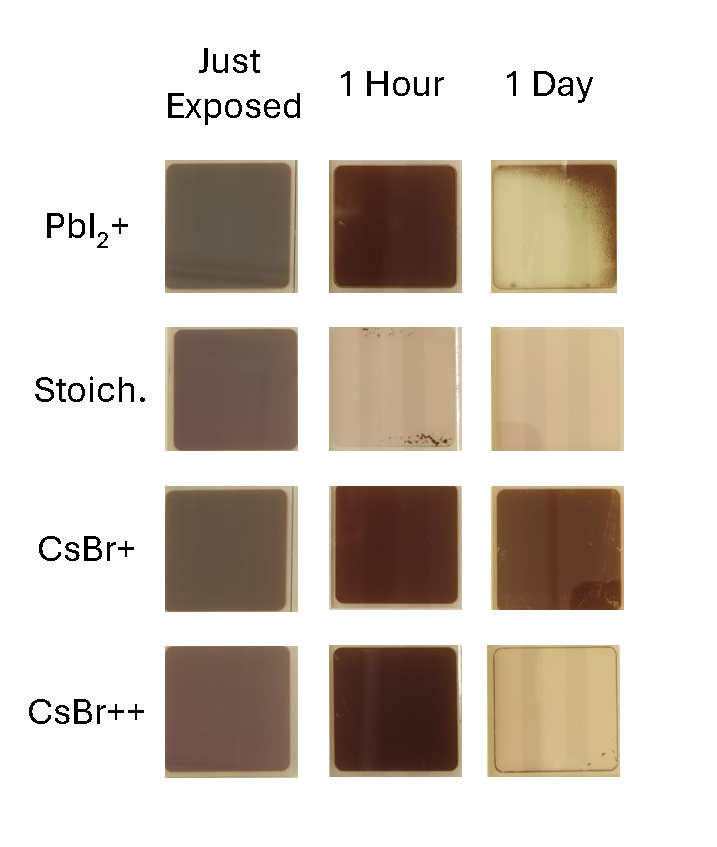
\includegraphics[width=\textwidth]{chapters/stability/imeges/Stability_Rotation_Stoichiometries.pdf} % Replace with your image file
        \caption*{(a)}
    \end{subfigure}
    \hfill
    \begin{subfigure}[t]{0.45\textwidth}
        \centering
        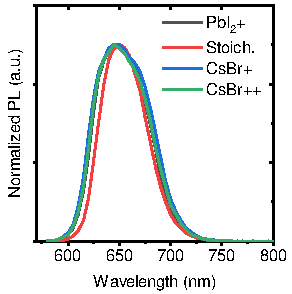
\includegraphics[width=\textwidth]{chapters/stability/imeges/PL_Normalized.pdf} % Replace with your image file
        \caption*{(b)}
    \end{subfigure}

    % Second row
    \begin{subfigure}[t]{0.99\textwidth}
        \centering
        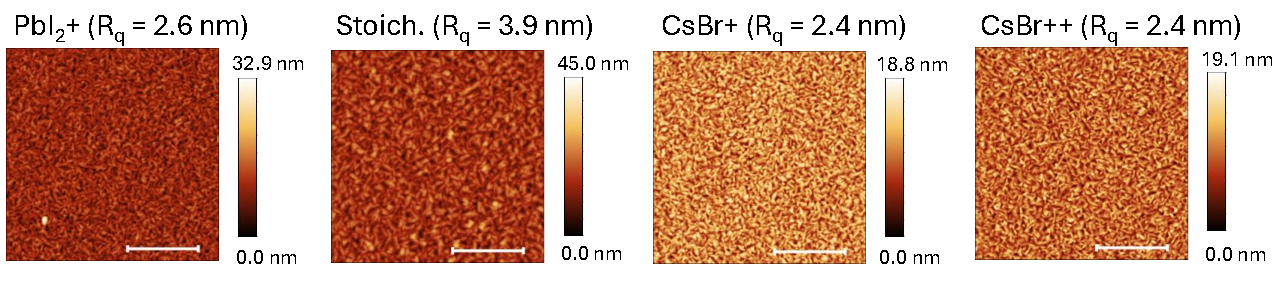
\includegraphics[width=\textwidth]{chapters/stability/imeges/Stability_Rotation_Stoich_AFM.pdf} % Replace with your image file
        \caption*{(c)}
    \end{subfigure}

    \caption{Characterization of (a) ambient stability, (b) SSPL spectra, and (c) surface morphology of \ch{CsPbI_2Br} thin films with various nominal CsBr:\ch{PbI_2} molar ratios.}
    \label{fig:stability:stoichiomtries_rotation}
\end{figure}

To investigate potential differences that could explain their varying ambient stability, we conducted PL and AFM measurements on one black-phase sample from each deposition condition. PL measurements show that all samples exhibit a similar emission peak at 645 nm with comparable full width at half-maximum (FWHM) (Figure~\ref{fig:stability:stoichiomtries_rotation}b). The only notable exception is the stoichiometric (Stoich.) sample, which displays a slightly red-shifted peak at 650 nm and a marginally narrower FWHM. The redshift of the emission peak could be a first indication of a \ch{PbI_2}-rich composition, contrary to the intended stoichiometry. On the other hand, there are no discernible differences among the other 3 samples that could potentially account for the superior stability of the CsBr+ sample one day after exposure. A similar trend is observed in the surface morphology of the 4 samples (Figure~\ref{fig:stability:stoichiomtries_rotation}c). The only sample that stands out is the Stoich. one, with slightly larger RMS roughness (3.9 nm compared to 2.6 and 2.4 nm), with the rest of the samples exhibiting an almost identical morphology. 


Since the optical and morphological properties of the samples did not sufficiently explain the ambient (in)stability of the deposited thin films, we employed Inductively Coupled Plasma Mass Spectrometry (ICP-MS) to investigate potential compositional differences. In ICP-MS, each sample is first digested in nitric acid to produce a homogeneous solution. This solution is then nebulized, vaporized, and ionized in a high-temperature argon plasma. The resulting ions are extracted and analyzed by a mass spectrometer, which identifies and quantifies them based on their mass-to-charge ratio. However, due to the poor ionization efficiency and volatility of halogens, it is not possible to accurately quantify iodine and bromine using this method. As a result, we focus on the measurable Cs:Pb mass ratio. Under the assumption that Cs originates solely from CsBr and Pb from \ch{PbI_2}, we can followingly use the Cs:Pb mass ratio to estimate the CsBr:\ch{PbI_2} molar ratio. Nevertheless, it should be noted that the measurement results are prone to errors, mainly introduced by the operator. Such errors can be appear, for instance, during the extrapolation of the calibration curve, the preparation of standard solutions and necessary dilutions, or the weighing of the samples. This is the reason why the measurement is repeated 3 times, allowing us to exact a mean value and its standard deviation. Therefore, the presented results should be treated qualitatively and as way to identify differences among the samples, rather than a precise quantification of their elemental composition. 

\begin{figure}[htbp]
    \centering
    % Second row
    \begin{subfigure}[t]{0.65\textwidth}
        \centering
        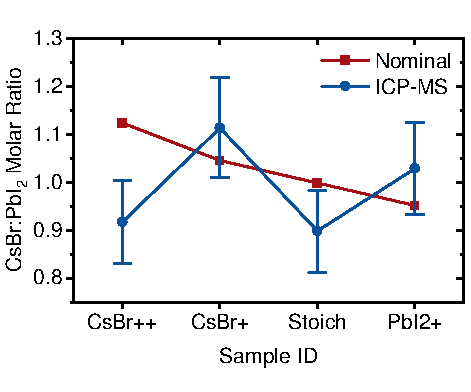
\includegraphics[width=\textwidth]{chapters/stability/imeges/Stability-ICP-MS.pdf} % Replace with your image file                
    \end{subfigure}

    \caption{Comparison of the nominal CsBr:\ch{PbI_2} molar ratio with the experimentally determined one, obtained through ICP-MS measurements.}
    \label{fig:stability:icp_ms}
\end{figure}

A comparison of the nominal and the ICP-derived precursor ratio for each deposition is presented in Figure~\ref{fig:stability:icp_ms}. Clearly, a significant divergence between the nominal and experimental stoichiometry is observed, particularly for samples CsBr++ and Stoich, both of which seem to have a \ch{PbI_2} rich composition. On the contrary, the sample CsBr+ contains the highest amount of CsBr. Although these results deviate significantly from the expected stoichiometric trend among the four samples, they may still offer a plausible explanation for the stability trend observed in Figure~\ref{fig:stability:stoichiomtries_rotation}. Specifically, and in line with previous literature, it is reasonable that the CsBr-rich sample (CsBr+ in this case) exhibits the highest stability, while the sample with the highest \ch{PbI_2} content (Stoich.) is the least stable one \cite{Ma2017TheCells}.

These results suggest that stoichiometry control is more challenging than initially presumed and cannot be reliably determined solely based on the evaporation rates of the two sources. They also highlight that the ambient stability of the samples is highly sensitive to even minor variations in precursor ratios—unlike device performance, which has been shown to be relatively tolerant to stoichiometric deviations (Figure~\ref{fig:etl_opt:molar_ratio}). In the exploration of factors that could affect the precise tuning of the deposited stoichiometry, we considered the lifetime of the QCMs, used to monitor the deposition rates of each source, as well as the condition of the precursor powders. While evaporation pressure could also be a contributing factor, all depositions were performed under high-vacuum conditions, with base pressures consistently below $6 \times 10^{-7}$ Torr (Table~\ref{tab:stability:stoichiometries}). At such pressures, the mean free path of the evaporated species exceeds 100 m, which is significantly greater than the distance between the crucibles and the substrates (Section~\ref{sec:materials_methods:fundamentals}), and thus should not limit the uniform transport of vapor to the substrate.

\begin{figure}[htbp]
    \centering
    % First plot
    \begin{subfigure}[t]{0.4\textwidth} % Adjust width as needed
        \centering
        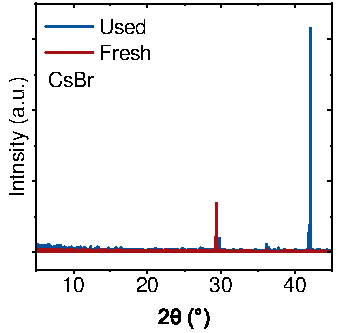
\includegraphics[width=\textwidth]{chapters/stability/imeges/CsBr_Powder.pdf} % Replace with your image
        \caption{}
        \label{}
    \end{subfigure}
    % Second plot
    \begin{subfigure}[t]{0.4\textwidth} % Adjust width as needed
        \centering
        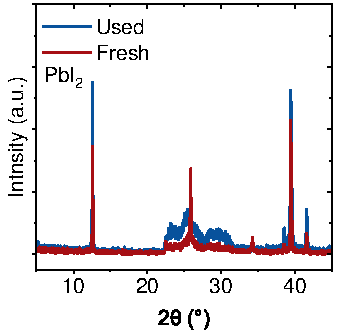
\includegraphics[width=\textwidth]{chapters/stability/imeges/PbI2_Powder.pdf} % Replace with your image
        \caption{}        
        \label{}
    \end{subfigure}

    % Caption for the whole figure
    \caption{Comparison of XRD patterns for (a) CsBr and (b) \ch{PbI_2} powders in their fresh state and after being used for a single thermal evaporation process.}   
    \label{fig:stability:fresh_used_powders}
\end{figure}

Before each deposition, the initial lifetime of the QCMs was consistently above 90\% (Table~\ref{tab:stability:stoichiometries}), and during the deposition itself it was dropping by approximately 4\% for the CsBr source and 9\% for the \ch{PbI_2} one. Considering the large drop in the lifetime of the \ch{PbI_2} sensor, a new rule was established to replace the QCM before each deposition to prevent potential discrepancies between the actual and measured deposition rates. The new protocol also involved using fresh precursor powder of consistent weight for each deposition. Prior to that, the same powder could be used for 2 or 3 consecutive depositions, considering that sufficient material was left in the crucible. In order to evaluate potential degradation of the precursor powder after one deposition, we submitted fresh and used CsBr and \ch{PbI_2} powders to X-Ray diffraction analysis (XRD)  (Figure~\ref{fig:stability:fresh_used_powders}). The measurement on \ch{PbI_2} powder revealed no major change in the position of the diffraction peaks, opposite to the CsBr powder, where the main peak shifted from 29.3\degree to 42\degree. Although the exact transformation of the material after cooling down from its vaporized state remains unclear, reusing the same powder could potentially alter its sublimation behavior and adsorption properties.


\subsection{Evaluation of Repeatability}

Based on the findings above, three additional depositions were performed (Table~\ref{tab:stability:stoichiometries_repeatbaility}) following a stricter protocol. This revised approach involved using fresh powder for each deposition and a new QCM for each source. Two of the depositions (A1 and A2), intended to be identical, targeted for a CsBr:\ch{PbI_2} molar ratio of 1.06:1.00. A third deposition (B1) aimed to evaluate the stability of films with a higher CsBr content, targeting a nominal ratio of 1.11:1.00. Four coupons were exposed for depositions A1 and A2, in order to assess potential dependence of the ambient stability on the substrate holder position.


\begin{table}[ht]
\centering
\caption{Summary of thermal evaporation parameters for the evaluation of ambient stability repeatability.}
\small % Reduce font size so it fits page width
\begin{tabular}{|
  >{\centering\arraybackslash}p{1.4cm} |
  >{\centering\arraybackslash}p{1.7cm} |
  >{\centering\arraybackslash}p{1.1cm} |
  >{\centering\arraybackslash}p{1.1cm} |
  >{\centering\arraybackslash}p{1.1cm} |
  >{\centering\arraybackslash}p{1.1cm} |
  >{\centering\arraybackslash}p{1.4cm} |
}
\hline
\makecell{\textbf{Dep. ID}} &
\makecell{\textbf{Nominal} \\ \textbf{CsBr:\ch{PbI_2}}} &
\makecell{\textbf{CsBr} \\ \textbf{Xtal} \\ {\%}} &
\makecell{\textbf{\ch{PbI_2}} \\ \textbf{Xtal} \\ {\%}} &
\makecell{\textbf{CsBr} \\ \textbf{Rate} \\ {\AA/s}} &
\makecell{\textbf{\ch{PbI_2}} \\ \textbf{Rate} \\ {\AA/s}} &
\makecell{\textbf{Evap.} \\ \textbf{Press.} \\ {Torr}} \\
\hline
A1     & 1.06:1.00 & 98.4 & 98.8 & 0.32 & 0.47 & $1\times10^{-7}$ \\
A2      & 1.06:1.00 & 98.4 & 98.5 & 0.32 & 0.47 & $1\times10^{-7}$ \\
B1      & 1.11:1.00 & 98.7 & 98.8 & 0.33 & 0.46 & $2\times10^{-7}$ \\

\hline
\end{tabular}
\label{tab:stability:stoichiometries_repeatbaility}
\end{table}

Figure~\ref{fig:stability:repeatability}a shows a schematic of the substrate holder, with sample positions labeled as S1 through S9. Each position has dimensions of $3\times3$ cm\textsuperscript{2}. Figure~\ref{fig:stability:repeatability}b and c illustrate the ambient stability of four samples from depositions A1 and A2, that were place on position S6, S7, S8, and S9. Despite following a stricter protocol, variations in ambient stability are still observed between the two, theoretically identical, depositions. Moreover, noticeable differences in stability also occur among samples within the same deposition. For instance, let's consider deposition A1 and the condition of the samples on the fourth day of exposure. Sample S8 is still in the black phase, samples S6 and S9 have almost fully converted to the yellow phase, while sample S7 has started showing signs of partial conversion. In contrary, the samples that came from deposition A2 were all almost fully converted by day 4. Additionally, sample S7, which was one of the most stable ones in deposition A1, started converting already in day 3. Even more unexpectedly, sample S9 of deposition B1, which was meant to have higher contents of CsBr and thus be more stable, was already fully converted to the yellow phase within one day of exposure. 


\begin{figure}[htbp]
    \centering
    % Second row
    \begin{subfigure}[t]{0.99\textwidth}
        \centering
        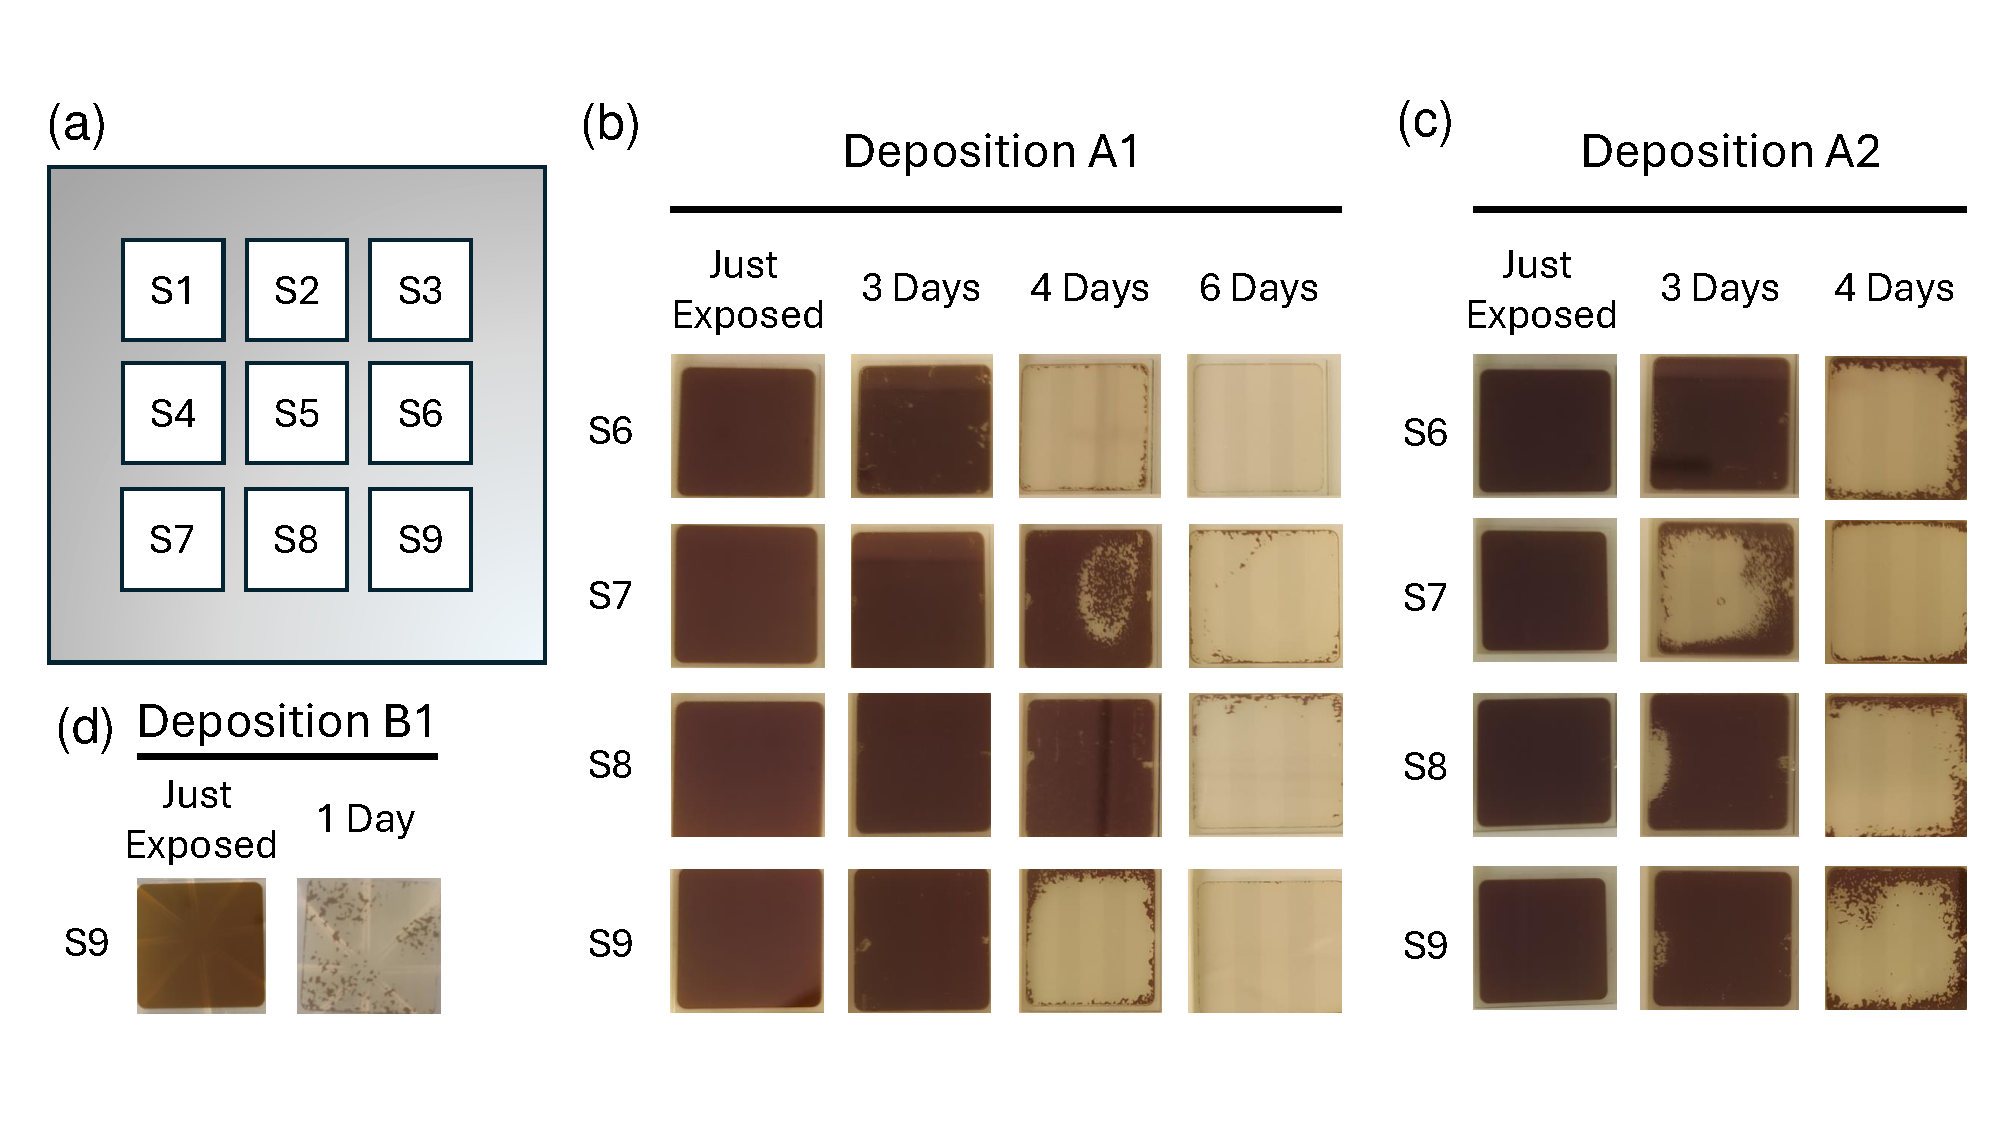
\includegraphics[width=\textwidth]{chapters/stability/imeges/Stability - Rotation.pdf} % Replace with your image file                
    \end{subfigure}
    \caption{(a) Schematic illustration of the substrate holder that can be loaded with up to nine $3\times 3$ $cm^2$ substrates. The position of each substrate on the holder is labeled as S1 to S9. Ambient stability of four samples from two, in principle, identical depositions, labeled as (b) A1 and (c) A2. The nominal CsBr:\ch{PbI_2} molar ratio was 1.05:1.00 for both. (d) Ambient stability of sample S9 from Deposition B1, which had a nominal CsBr:\ch{PbI_2} molar ratio equal to 1.1:1.0.}
    \label{fig:stability:repeatability}
\end{figure}

These results emphasize that even with a stricter protocol in terms of precursor powder and QCM usage, it is not possible to accurately predict and control the ambient stability of the \ch{CsPbi_2Br} thin films. One thing that can be excluded though is the potential sensitivity of ambient stability to the position of a sample within the substrate holder. It is likely that additional, less controllable, factors significantly influence the stability of the deposited films. These factors may include substrate preparation details, such as potential contamination between the cleaning process and transfer to the vacuum chamber, as well as conditions within the chamber itself. For instance, material buildup on the chamber walls might alter evaporation dynamics and affect film uniformity or composition. In any case, this study highlights the limited reproducibility of ambient stability experiments, at least in the context of thermally evaporated perovskite thin films. This finding stands in contrast to a common practice in literature, where stability data are often reported for only a small number of samples, potentially only the best-performing ones, without providing information on the repeatability of the results. Consequently, a more critical evaluation of reported findings in this field is essential.

In the framework of this thesis, many efforts were dedicated to achieving a consistent improvement in the ambient stability of the \ch{CsPbI_2Br} thin films. Such efforts included the tuning of the total deposition rate, the annealing temperature, duration and environment, as well as the introduction of template layers (such as a thin layer of CsBr) on top or below the perovskite lattice. These strategies were guided by previously published studies, primarily focused on solution-processed films. Nevertheless, none of these approaches resulted in a repeatable ambient stability that consistently exceeded 48 hours.


\section{Assessment of Ambient Stability via Combinatorial Depositions}

The lack of repeatability and control over the ambient stability of the thermally co-evaporated \ch{CsPbI_2Br} thin films necessitates multiple depositions under identical conditions to obtain meaningful statistical estimations. However, this considerably extends the time-frame of related experiments. For instance, for a single deposition run, during which only one set of parameters can be evaluated, time must be allocated for the evaporation process itself ($\approx$ 2 hr), as well as for the vacuum pump-down ($\approx$ 2 hr) and the post-deposition source-cooling before the chamber can be safely vented ($\approx$ 3 hr). In some cases, and as shown in the previous section, the stability of the samples themselves lasts as long as the time required for their preparation (about 1 day), creating a significant bottleneck in research progress in this domain.  

\begin{figure}[htbp]
    \centering
    % First plot
    \begin{subfigure}[t]{0.49\textwidth} % Adjust width as needed
        \centering
        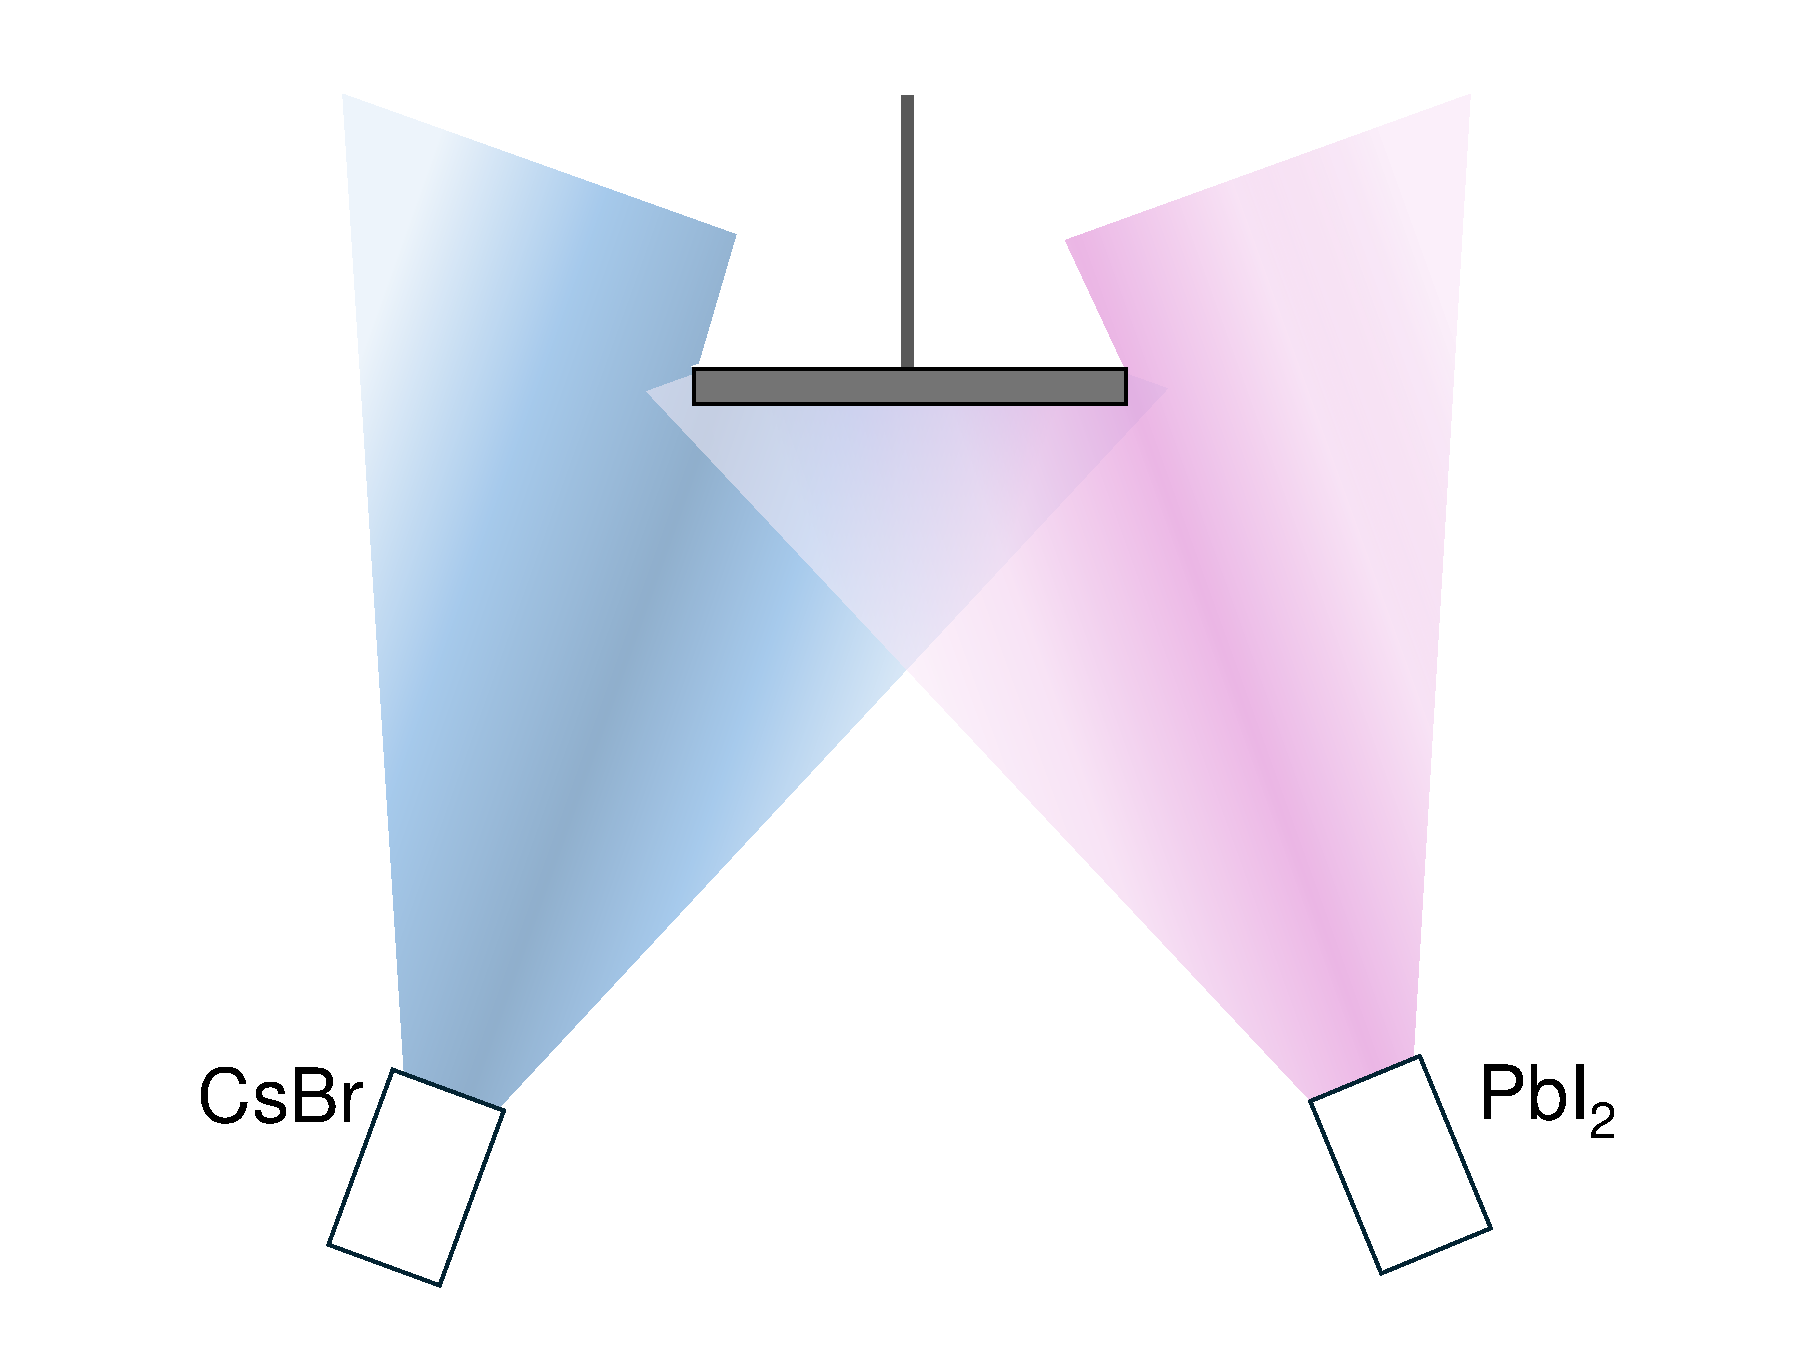
\includegraphics[width=\textwidth]{chapters/stability/imeges/Chamber - Side View.pdf} % Replace with your image
        \caption{}
        \label{}
    \end{subfigure}
    % Second plot
    \begin{subfigure}[t]{0.49\textwidth} % Adjust width as needed
        \centering
        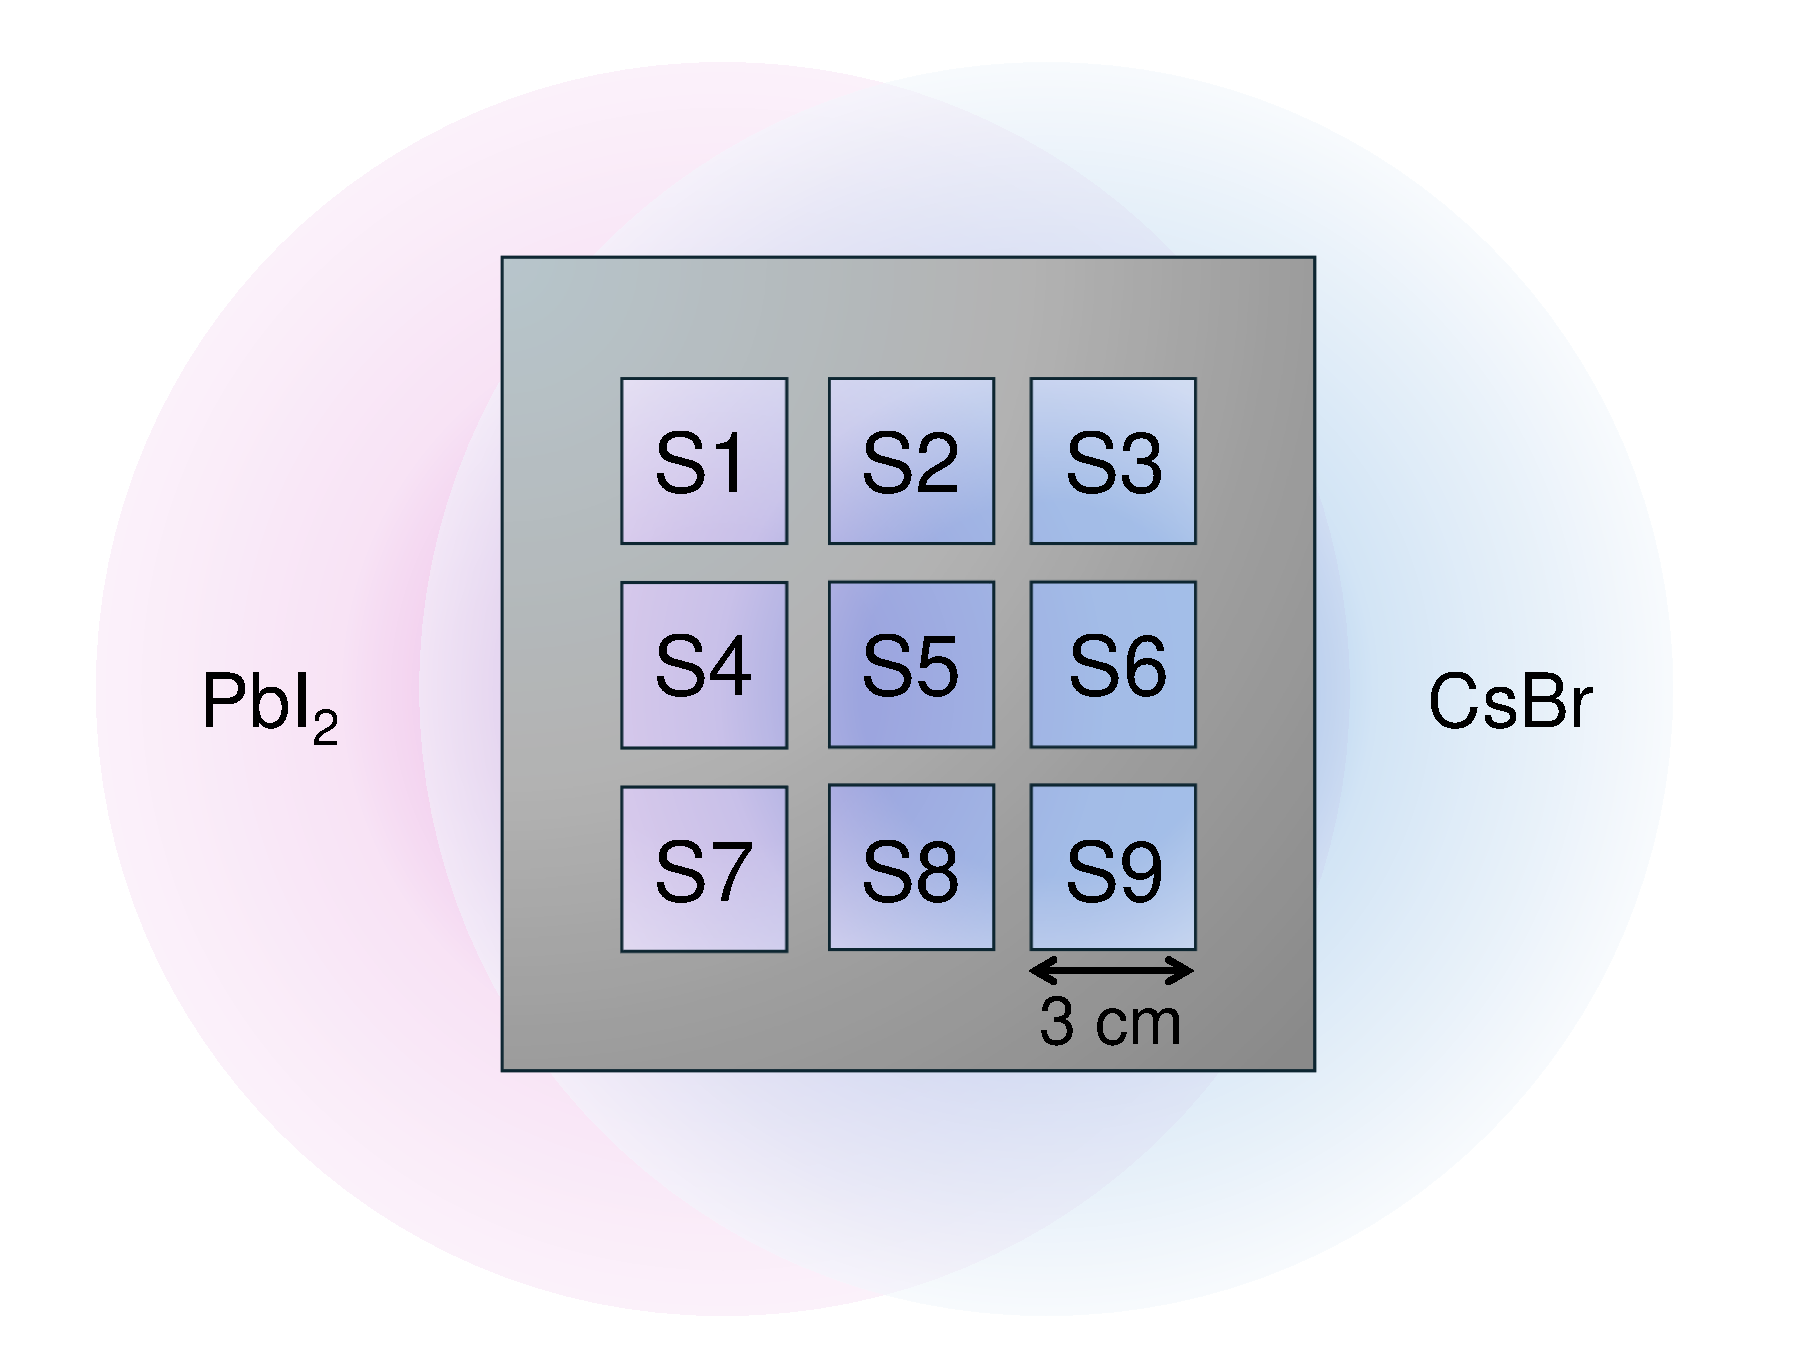
\includegraphics[width=\textwidth]{chapters/stability/imeges/Holder - Gradient - Schematic.pdf} % Replace with your image
        \caption{}        
        \label{}
    \end{subfigure}

    % Caption for the whole figure
    \caption{(a) Schematic representation of the vapor flux profile, illustrating higher intensity along the central axis and decreasing flux at larger angles from the source. When the rotation of the substrate holder is de-activated, this leads to (b) a gradient of perovskite compositions across the substrate holder. The position of the CsBr and \ch{PbI_2} sources with respect to the substrate holder is only a visual representation and does not represent the real arrangement inside the vacuum chamber.}   
    \label{fig:stability:combinatorial_approach}
\end{figure}


In order to overcome this challenge, we evaluate the use of combinatorial thermal evaporation for high-throughput experimentation. Combinatorial material science (CMS) has been widely utilized for the exploration and the development of new materials with applications in catalysis, electronics, industrial coatings, sensing, and biology \cite{Potyrailo2011CombinatorialArt}. CMS for thin film exploration relies on modifying a deposition method so that a specific film parameter (such as the thickness or composition) is no longer constant across the substrate, but rather forms a continuous gradient. Followingly, the use of high-throughput characterization methods is necessary to characterize the spatial distribution of the film's properties, establishing a "library" of properties as function of the varied film parameter \cite{McGinn2019Thin-filmReview, Xiang1999CombinatorialMaterials, Ludwig2019DiscoveryMethods}. Such an approach has been already used in the field of perovskite research. For instance, Näsström et al. utilized combinatorial inkjet printing to study the phase transition temperatures of \ch{CsPbBr_xI_{3-x}} thin films \cite{Nasstrom2020DependenceExperimentation}. A compositional gradient was achieved by using an inkjet printer with two different print-heads, which were programmed to print an image with varying coverage across the substrate. In terms of thermal co-evaporation, CMS can be achieved by simply disabling the rotation of the substrate folder, allowing for the formation of compositional or thickness gradients across the film  \cite{Becker2019LowExperimentation, Susic2023CombinatorialCells, Lin2024FormationTreatment, Huang2021Vapor-deposited16, Li2019High-ThroughputDeposition}. In what regards the study of \ch{CsPbI_x_Br_{3-x}}  (for x= 1 or 2) perovskites, it has already been established that a clear boundary exists between the Pb-rich and Cs-rich region of the as-deposited films \cite{Becker2019LowExperimentation, Huang2021Vapor-deposited16, Lin2024FormationTreatment}. However, the impact of compositional variation on the ambient stability of the films remains largely unexplored. For this reason, we adopt a combinatorial approach for the co-evaporation of CsBr and \ch{PbI_2} (Figure~\ref{fig:stability:combinatorial_approach}a), with a representation of the compositional gradient illustrated in Figure~\ref{fig:stability:combinatorial_approach}b.


\subsection{Large Area Stoichiometry Mapping}


\begin{figure}[ht!]
    \centering
    % First row
    \begin{subfigure}[t]{0.49\textwidth}
        \centering
        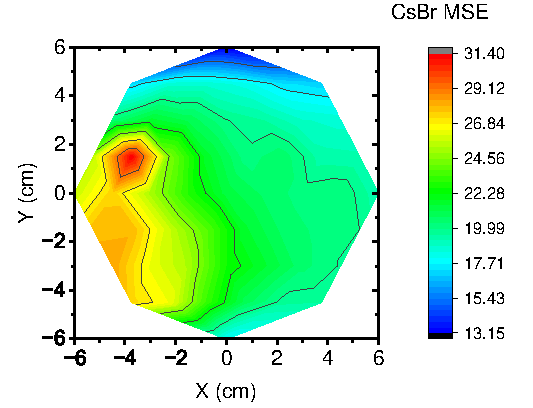
\includegraphics[width=\textwidth]{chapters/stability/imeges/CsBrMSE.pdf} % Replace with your image file
        \caption*{(a)}
    \end{subfigure}
    \hfill
    \begin{subfigure}[t]{0.49\textwidth}
        \centering
        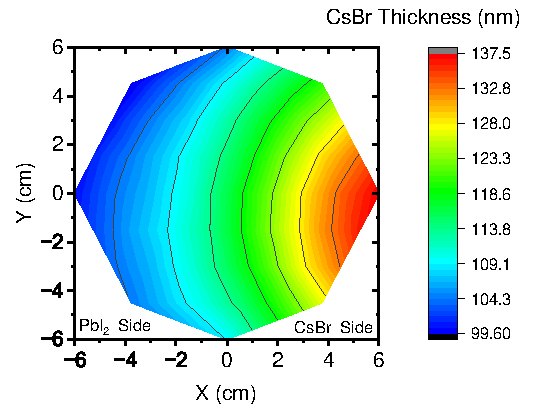
\includegraphics[width=\textwidth]{chapters/stability/imeges/CsBrThickness.pdf} % Replace with your image file
        \caption*{(b)}
    \end{subfigure}


    % Second row
    \begin{subfigure}[t]{0.49\textwidth}
        \centering
        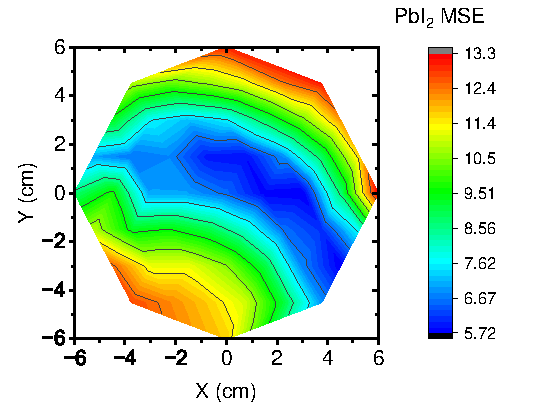
\includegraphics[width=\textwidth]{chapters/stability/imeges/PbI2MSE.pdf} % Replace with your image file
        \caption*{(c)}
    \end{subfigure}
    \hfill
    \begin{subfigure}[t]{0.49\textwidth}
        \centering
        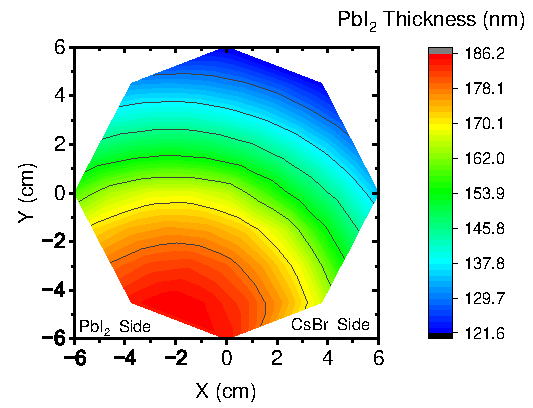
\includegraphics[width=\textwidth]{chapters/stability/imeges/PbI2Thickness.pdf} % Replace with your image file
        \caption*{(d)}
    \end{subfigure}
    \caption{Spectroscopic ellipsometry results showing (a) the fitting MSE and (b) the spatial thickness distribution of the CsBr layer following its deposition on a 6-inch wafer. Spectroscopic ellipsometry results showing (c) the fitting MSE and (d) the spatial thickness distribution of the \ch{PbI_2} layer following its deposition on a 6-inch wafer.}
    \label{fig:stability:ellipsometry:thickness_mse}
\end{figure}

In order to evaluate the compositional gradient across the whole substrate holder during a combinatorial deposition, we replace the $3\times3$ $cm^2$ coupons with 6'' (or $\approx$ 15 cm) wafer. This way, it is possible to deposit each precursor on a separate wafer and use a high-throughput characterization technique, such as spectroscopic ellipsometry, to extract information about the precursor's continuous thickness variation across a large area. This approach is illustrated in Figure~\ref{fig:stability:ellipsometry:thickness_mse}. While the MSE of model developed for the \ch{PbI_2} layer is maintained below 14 across the whole wafer (Figure~\ref{fig:stability:ellipsometry:thickness_mse}c), the deviation between experimental and simulated results is larger in the case of the CsBr layer (MSE is beyond 30 in certain areas in Figure~\ref{fig:ellipsometry:roughness_thickness}a). This is attributed to the hygroscopic nature of alkali halides and the fact that cesium halides' surface transitions from a transparent and reflective one to a rough and diffusive one within minutes of exposure to ambient moisture \cite{Chen2017All-Vacuum-Deposited11}. Nevertheless, there is a good agreement between the nominal thickness of each precursor (111 nm for CsBr and 164 nm for \ch{PbI_2}) and the modeled thickness in the center of each wafer (116 nm and 165 nm in Figure~\ref{fig:stability:ellipsometry:thickness_mse}b and d, respectively). Simultaneously, the iso-concentration lines for the thickness variation of each precursor exhibit a radial symmetry, with the thickness maxima indicating the position of the respective source crucible relative to the wafer holder. 

\begin{figure}[htbp]
    \centering
    % First row
    \begin{subfigure}[t]{0.6\textwidth}
        \centering
        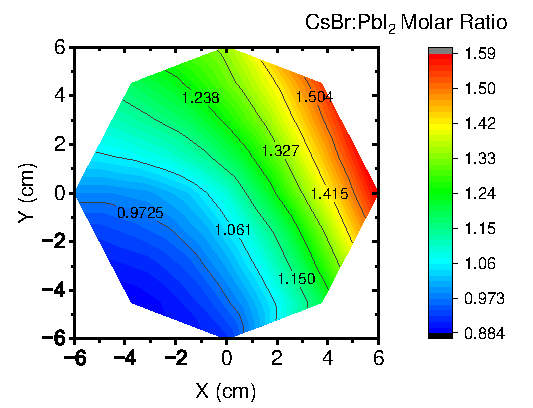
\includegraphics[width=\textwidth]{chapters/stability/imeges/Molar_Ratio.pdf} % Replace with your image file
        \caption*{(a)}
    \end{subfigure}
    \begin{subfigure}[t]{0.25\textwidth}
        \centering
        \raisebox{1.5cm}{ % Adjust this value to move the image up or down
            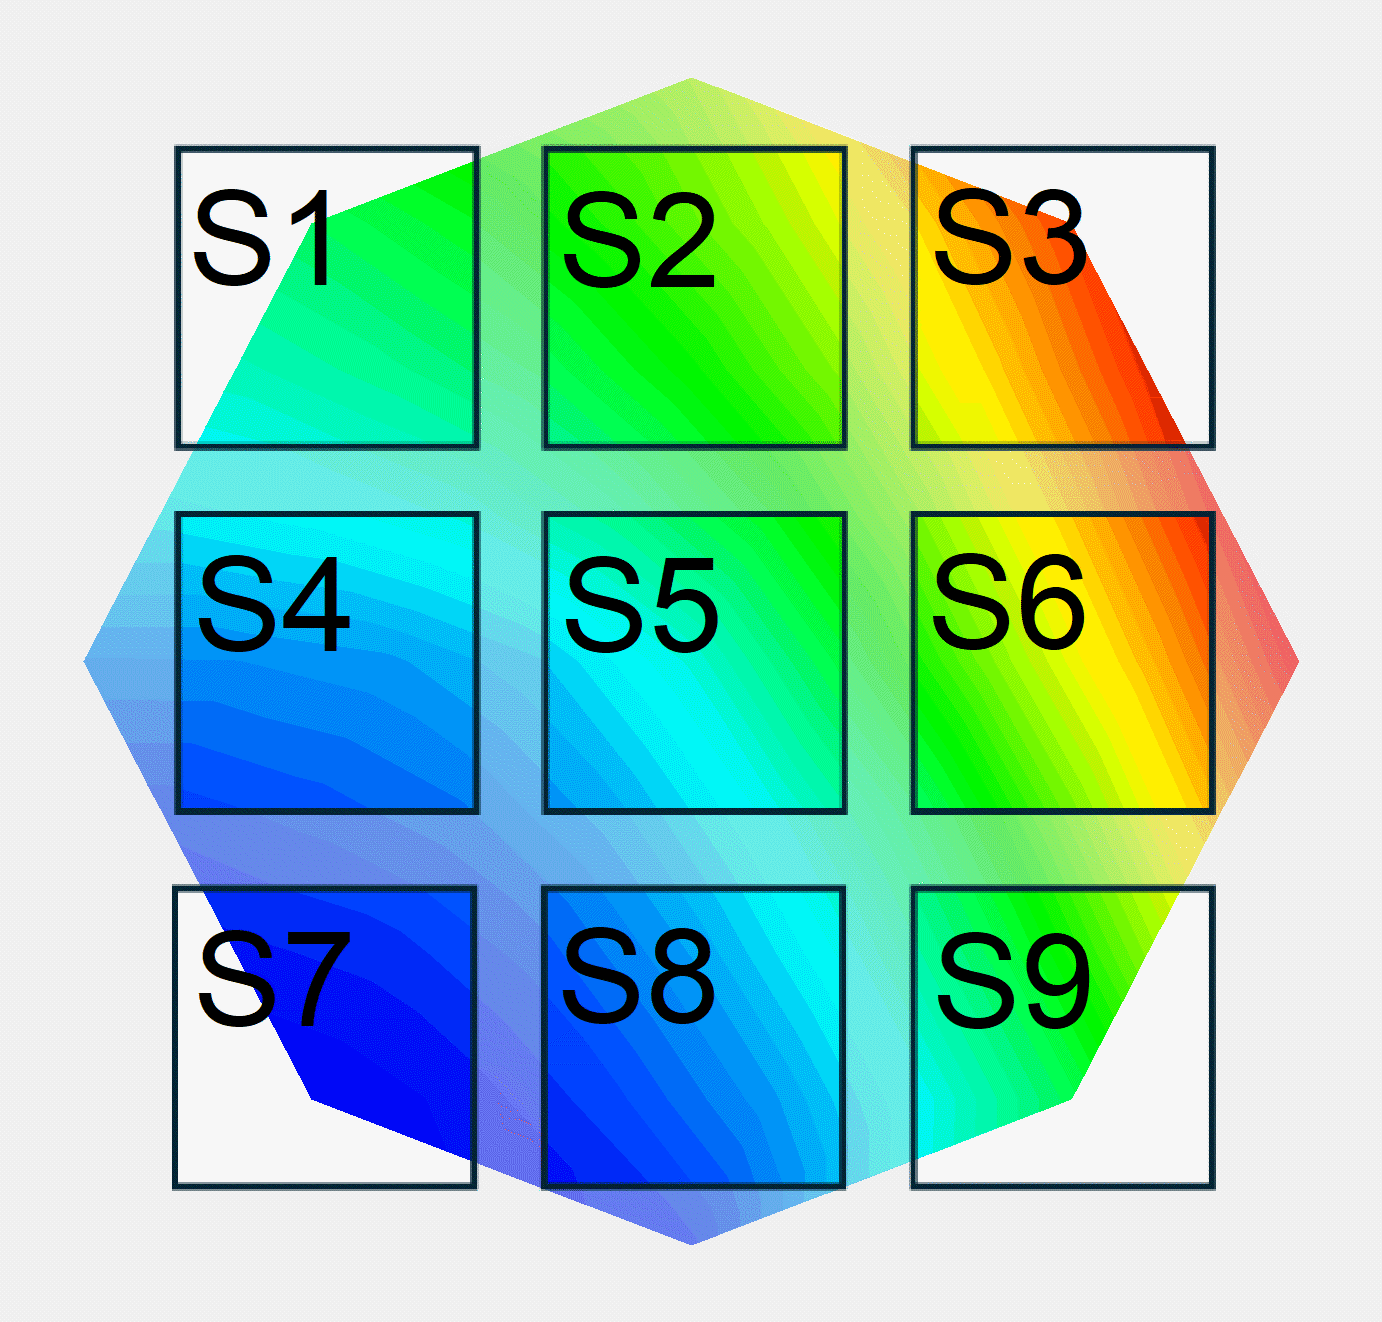
\includegraphics[width=\textwidth]{chapters/stability/imeges/Molar_Ratio_on_Substrate.png}
        } % Replace with your image file
        \caption*{(b)}
    \end{subfigure}

\caption{(a) Spatial distribution of the CsBr to \ch{PbI_2} molar ratio across the 6-inch wafer. (b) Overlay comparison of the substrate holder and compositional spatial distribution.}
\label{fig:stability:ellipsometry:molar_ratio}

\end{figure}


Based on the thickness variations of the two precursors, it is possible to analytically calculate the distribution of the CsBr to \ch{PbI_2} molar ratio across the whole wafer, as shown in Figure~\ref{fig:stability:ellipsometry:molar_ratio}a. The nominal range of the CsBr:\ch{PbI_2} ratio varies between approximately 0.88:1.00 and 1.6:1.00. Lastly, Figure~\ref{fig:stability:ellipsometry:molar_ratio}b provides a visual representation of the correspondence between the wafer map and the position of the individual $3\times3$ $cm^2$ coupons.
 

\subsection{Impact of Substrate Type and Perovskite Thickness}

Continuing with the combinatorial deposition approach, we performed three co-evaporations on $3\times3$ $cm^2$ coupons, with the following characteristics: (i) 300 nm of a \ch{CsPbI_2Br} layer on glass substrates (Figure~\ref{fig:stability:no_rotation:300nm_glass}), (ii) 150 nm of a \ch{CsPbI_2Br} layer on glass substrates (Figure~\ref{fig:stability:no_rotation:150nm_glass}), and (iii) 300 nm of a \ch{CsPbI_2Br} layer on glass/ITO/NiO substrates (Figure~\ref{fig:stability:no_rotation:300nm_ito_nio}). In all cases, the nominal CsBr:\ch{PbI_2} molar ratio (i.e. the intended ratio at the center of the substrate holder) was equal to 1.05:1.00. The first two depositions aimed to evaluate the impact of perovskite thickness on the ambient stability of the films, as it can be expected that with increasing thickness, the relative volume of the perovskite film that is subject to surface strain will decrease \cite{Steele2019ThermalFilms}. On the other hand, the third deposition focused on assessing the influence of the substrate on ambient stability, specifically the type of substrate used in device fabrication, since it has been previously shown that it can have a drastic impact on not only the strain on the perovskite lattice, but also its preferential orientation \cite{Abzieher2021FromCells, Xue2020RegulatingLayers}. All 9 samples from each deposition run were flash annealed at 300\degree C in nitrogen environment, before being exposed and stored in ambient conditions. 


\begin{figure}[htbp]
    \centering
    % Second row
    \begin{subfigure}[t]{0.99\textwidth}
        \centering
        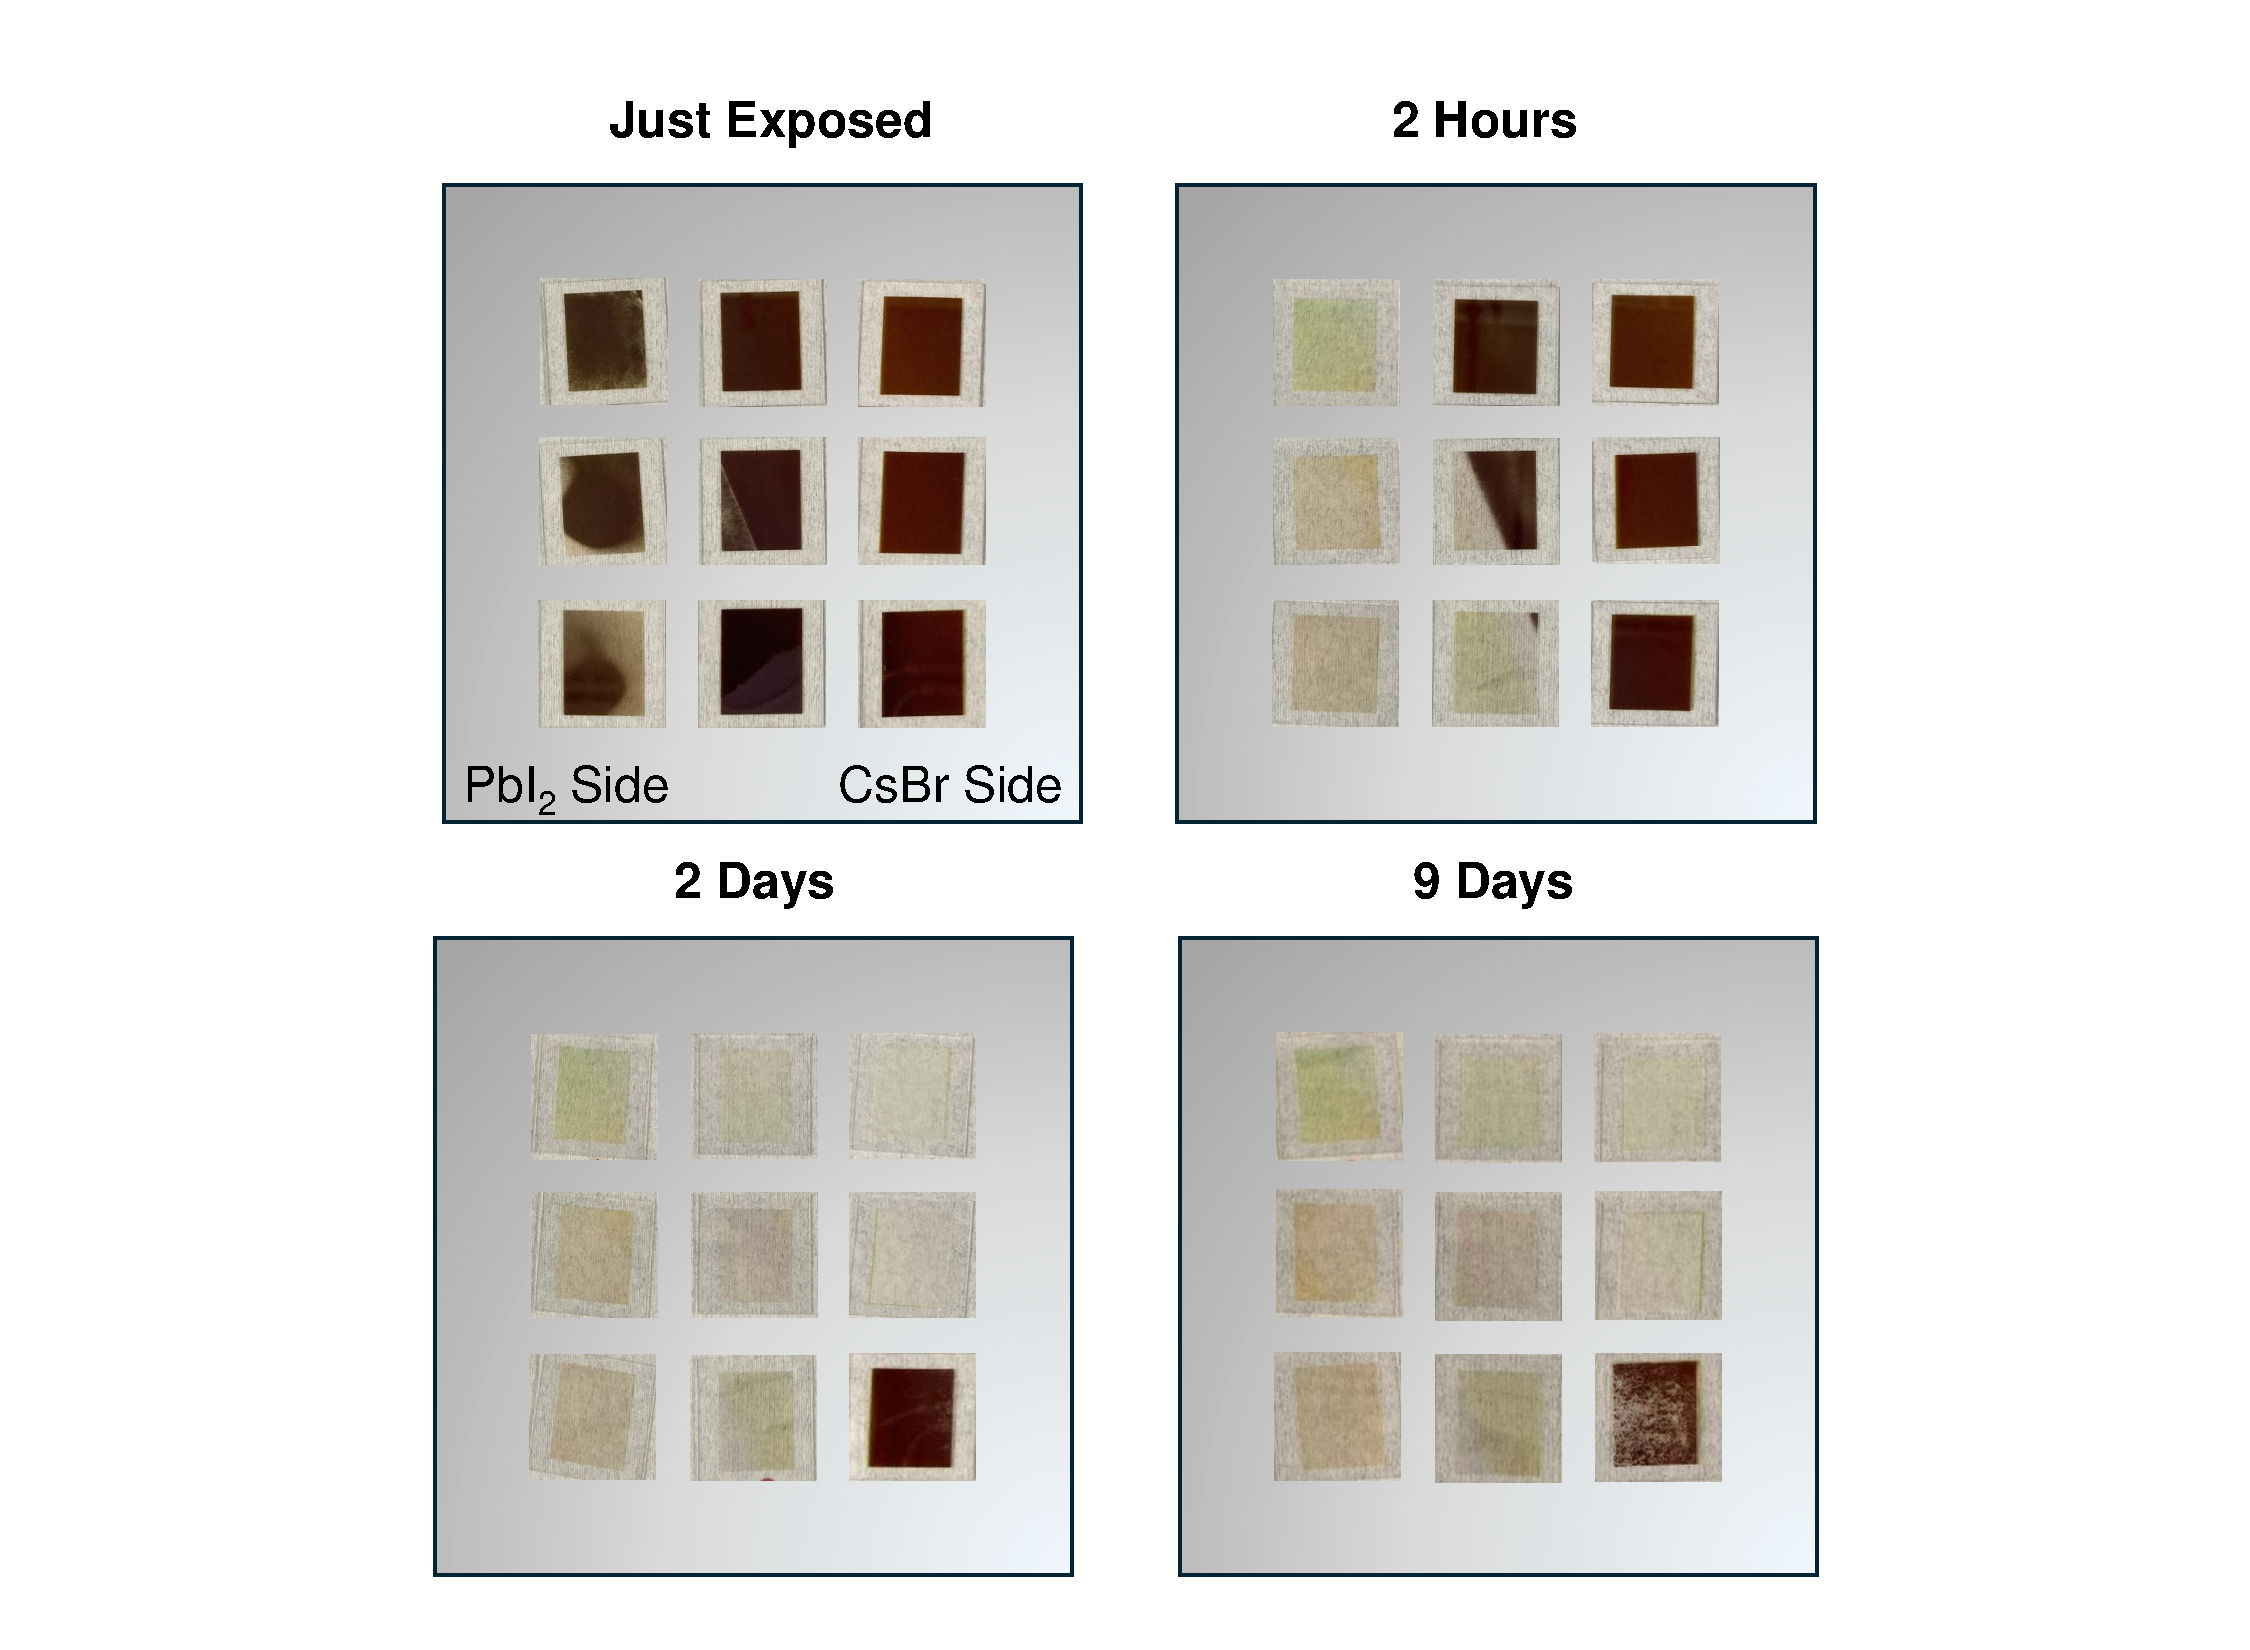
\includegraphics[width=\textwidth]{chapters/stability/imeges/Stability - No Rotation_275nm_on_glass.pdf} % Replace with your image file
               
    \end{subfigure}

    \caption{Ambient stability of 300-nm-thick \ch{CsPbI_2Br} thin films deposited via combinatorial co-evaporation on glass substrates.}
    \label{fig:stability:no_rotation:300nm_glass}
\end{figure}


The ambient stability of samples with 300 nm of \ch{CsPbI_2Br} films on glass substrates is shown in Figure~\ref{fig:stability:no_rotation:300nm_glass}. Within just a few hours of exposure to ambient moisture, two distinct regions emerge, characterized by black and yellow phases with a clearly defined phase boundary. By comparing the position of this boundary with the spatial distribution of the CsBr:\ch{PbI_2} molar ratio at the wafer level, as well as with findings from previous studies \cite{Becker2019LowExperimentation, Lin2024FormationTreatment}, we conclude that the boundary lies on the stoichiometrically-balanced region of the film, separating the Pb-rich (less stable) region from the Cs-rich (more stable) one. Interestingly, while previous reports observed a sharp boundary in as-deposited films, we find that the boundary remains distinctly sharp even after flash-annealing at 300\degree C, despite the diffusion likelihood of the perovskite's constituent elements. Two days after exposure, only the film in the bottom right remains in the black phase, though it also begins to convert by the ninth day.


\begin{figure}[htbp]
    \centering
    % Second row
    \begin{subfigure}[t]{0.99\textwidth}
        \centering
        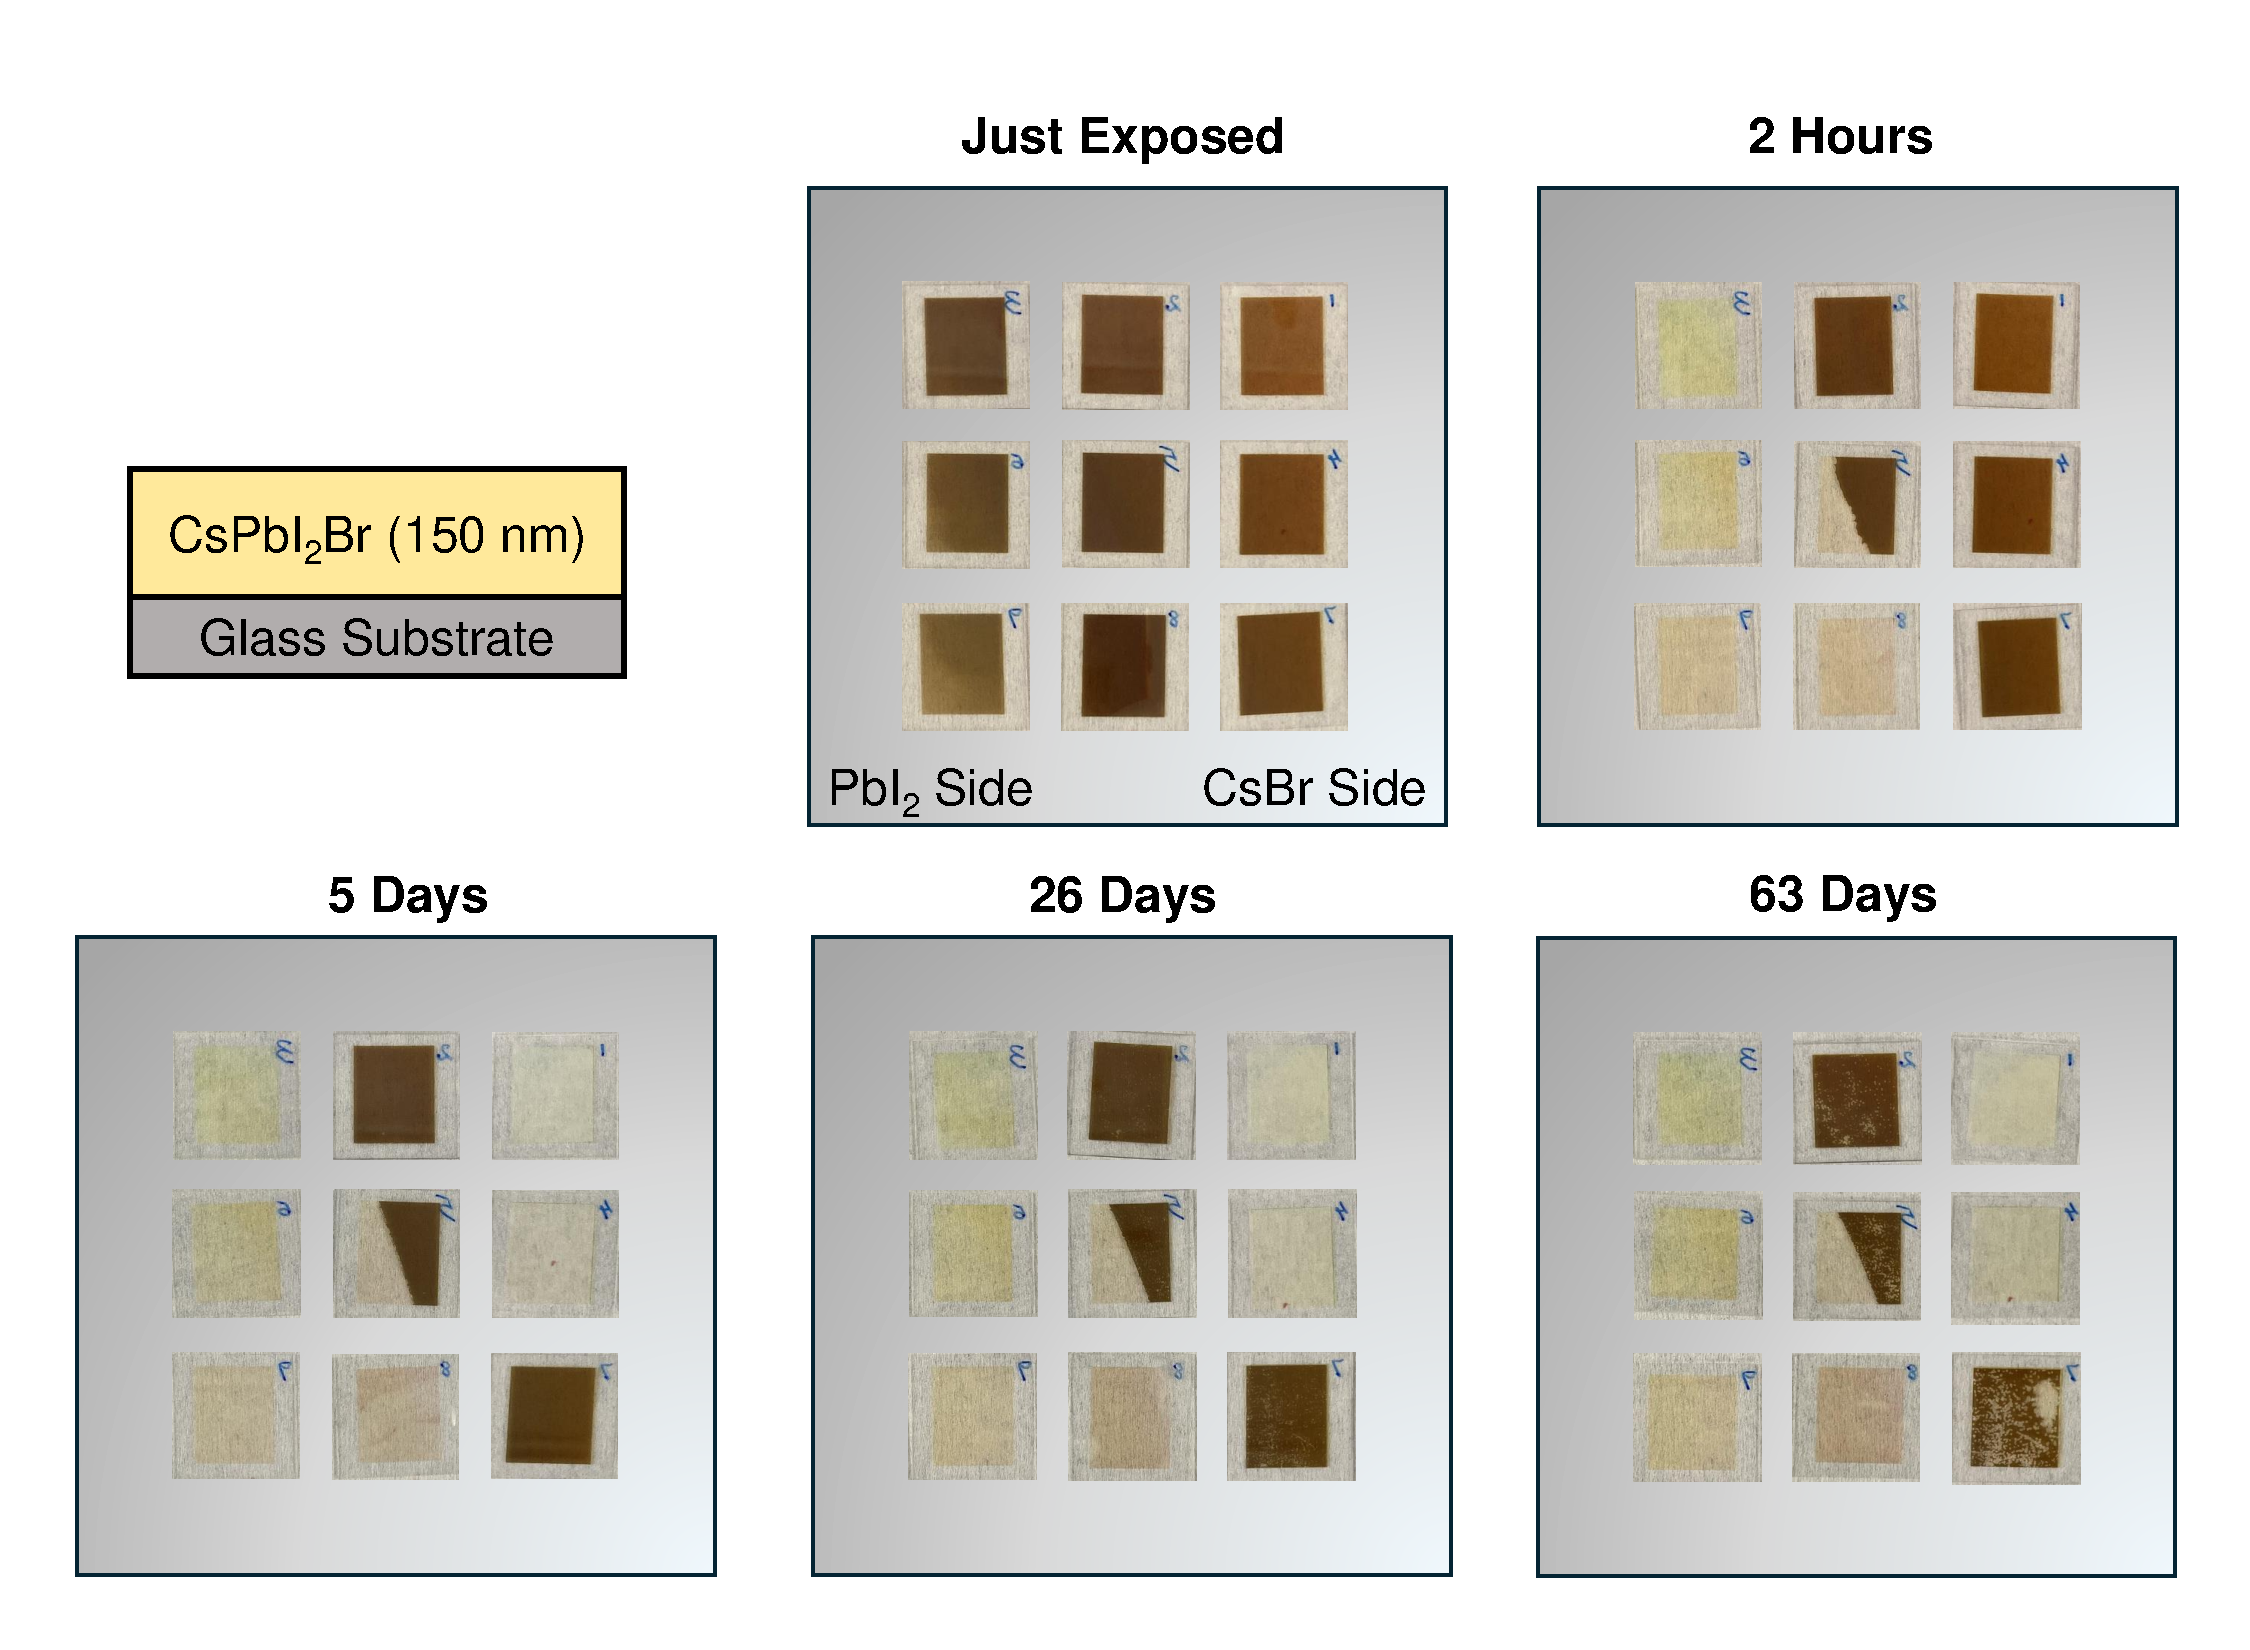
\includegraphics[width=\textwidth]{chapters/stability/imeges/Stability_No_Rotation_139nm_on_glass.pdf} % Replace with your image file                
    \end{subfigure}

    \caption{Ambient stability of 150-nm-thick \ch{CsPbI_2Br} thin films deposited via combinatorial co-evaporation on glass substrates.}
    \label{fig:stability:no_rotation:150nm_glass}
\end{figure}

Reducing the thickness of the perovskite film to half does not delay the conversion of the Pb-rich region within the first two hours of exposure to the ambient moisture (Figure~\ref{fig:stability:no_rotation:150nm_glass}). However, it does was have a significant impact on the stability of the Cs-rich region over the course the following days. Specifically, the samples just on the right side of the phase boundary maintain their stability for more than 26 days, starting to show signs of conversion only 63 days after their exposure. Comparing the position of the most stable samples with the distribution of the CsBr:\ch{PbI_2} moalr ratio in Figure~\ref{fig:stability:ellipsometry:molar_ratio}, it can be deduced that their CsBr:\ch{PbI_2} molar ratio approximately varies between 1.15:1.00 and 1.35:1.00. This experiment highlights that increasing the CsBr content beyond a certain threshold begins to negatively impact film stability, whereas reducing the film thickness by half can enhance stability, extending it to a timescale of several months.

\begin{figure}[htbp]
    \centering
    % Second row
    \begin{subfigure}[t]{0.99\textwidth}
        \centering
        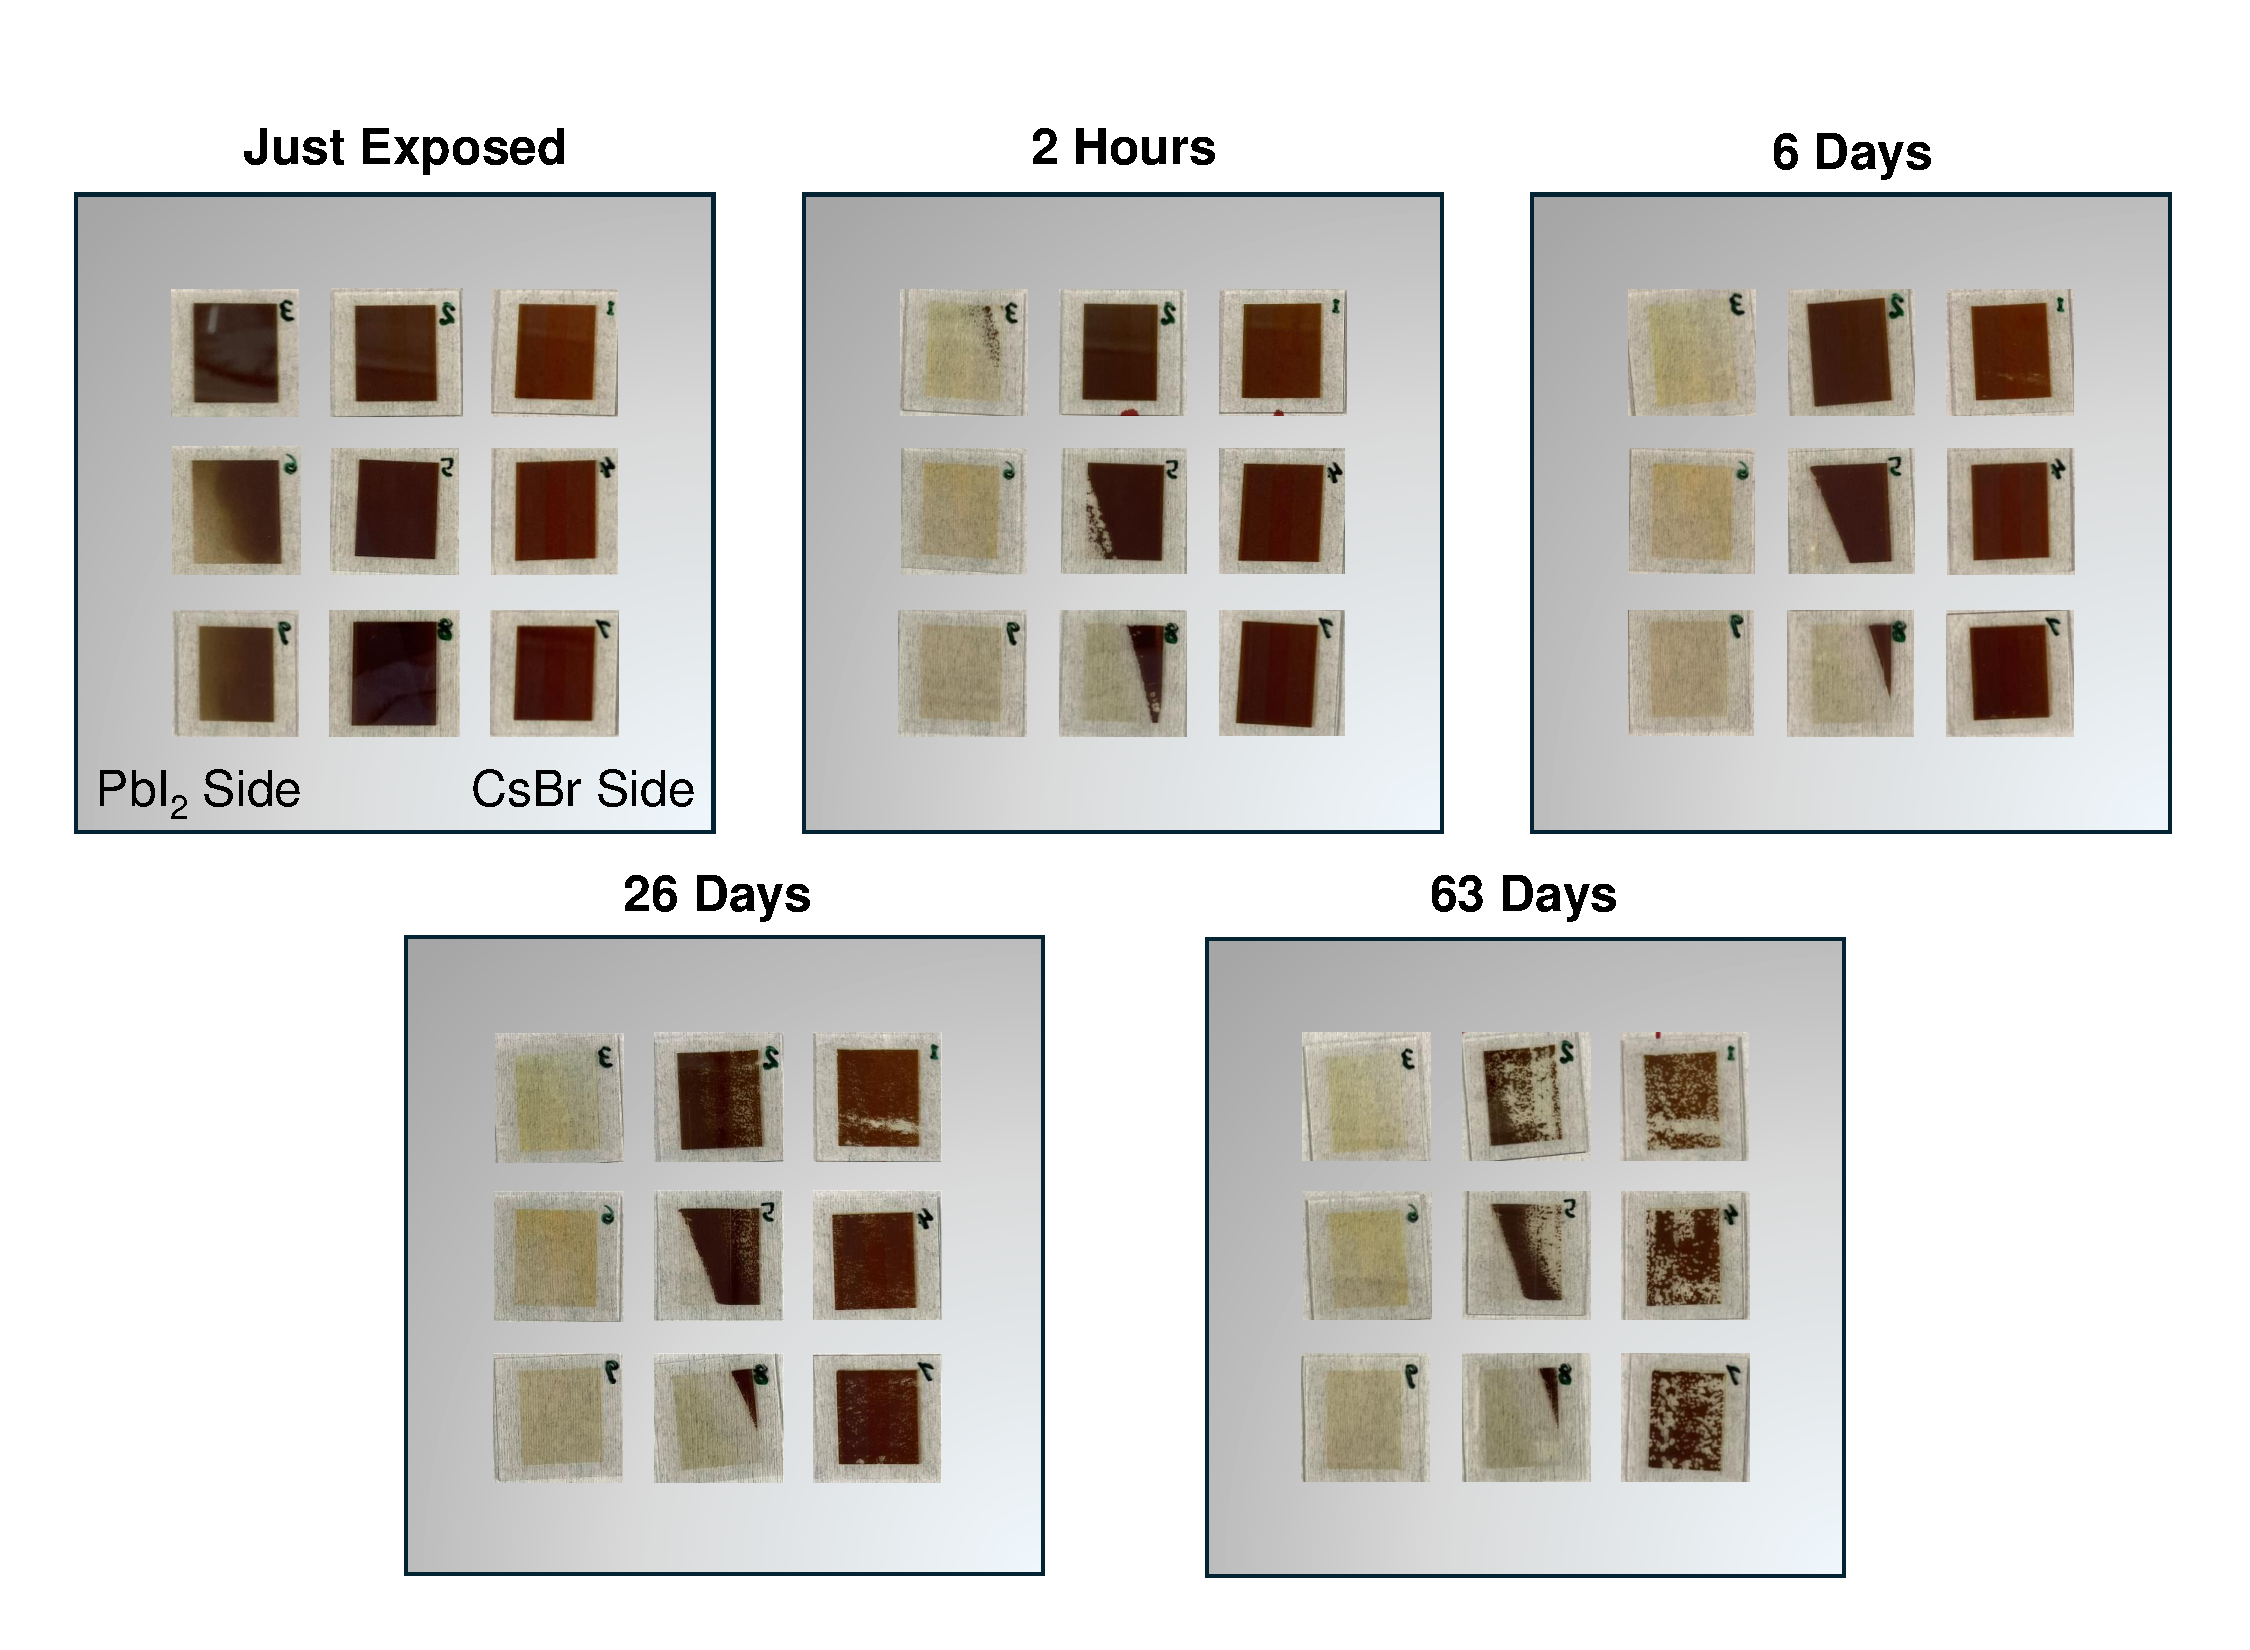
\includegraphics[width=\textwidth]{chapters/stability/imeges/Stability_No_Rotation_275_on_nio.pdf} % Replace with your image file                
    \end{subfigure}

    \caption{Ambient stability of 300-nm-thick \ch{CsPbI_2Br} thin films deposited via combinatorial co-evaporation on glass/ITO substrates, coated with 15 nm of \ch{NiO_x}.}
    \label{fig:stability:no_rotation:300nm_ito_nio}
\end{figure}


Lastly, Figure~\ref{fig:stability:no_rotation:300nm_ito_nio} demonstrates the stability of 300 nm \ch{CsPbI_2Br} films, deposited on glass/ITO substrates, coated with 15 nm on \ch{NiO_x}. The key difference in this case is that all samples on the right side of the phase boundary maintain their stability for over 26 days, even at a thickness of 300 nm. This further highlights the importance of the selected substrate on the ambient stability, which needs to be further evaluated in future experiments. To assess the repeatability of the experiment, an identical deposition was performed (Figure~\ref{fig:appendix:stability_on_NiO_v2}), demonstrating that all samples on the right side of the phase boundary remained stable for over six days. 

As a result, through the combinatorial thermal co-evaporation approach, and only three depositions, it was possible to gain valuable insights into factors that affect the ambient stability of \ch{CsPbI_2Br} thin films, including their composition, thickness, and substrate type. Nevertheless, additional characterization measurements are required to further explain and quantify the underlying physical mechanisms. An additional parameter that needs to be evaluated in future studies is the absence of rotation itself on the stability of the deposited films. The aforementioned depositions revealed that depositing films with a nominal CsBr:\ch{PbI_2} molar ratio in the range of 1.2:1.0 should, in principle, boost the stability of the films beyond a couple days. However, this result could not be reproduced for samples deposited with substrate rotation activated. This could hint towards a fundamentally different growth and crystallization mechanism of films deposited with and without rotation, that has a critical impact on the strain on the lattice and by extension to the ambient stability of the films. 


\subsection{Ambient Stability of PePDs}


\begin{figure}[ht!]
    \centering
    % First row
    \begin{subfigure}[t]{0.49\textwidth}
        \centering
        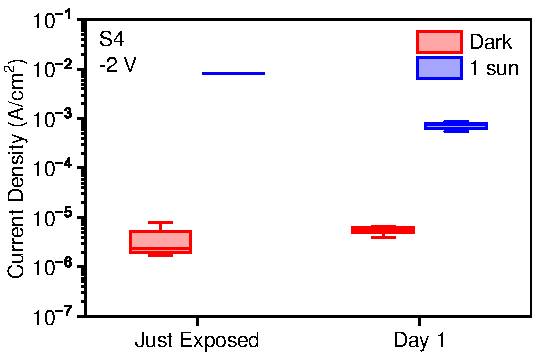
\includegraphics[width=\textwidth]{chapters/stability/imeges/AP44_6_Thesis.pdf} % Replace with your image file
        \caption*{(a)}
    \end{subfigure}
    \hfill
    \begin{subfigure}[t]{0.49\textwidth}
        \centering
        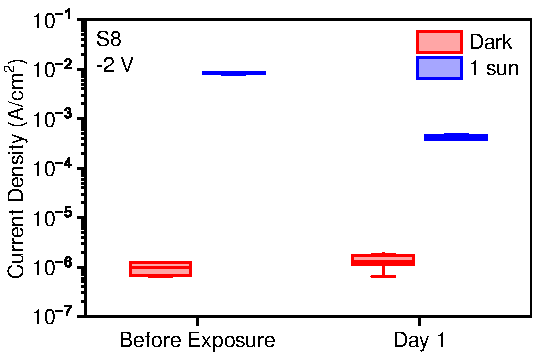
\includegraphics[width=\textwidth]{chapters/stability/imeges/AP44_8_Thesis.pdf} % Replace with your image file
        \caption*{(b)}
    \end{subfigure}


    % Second row
    \begin{subfigure}[t]{0.99\textwidth}
        \centering
        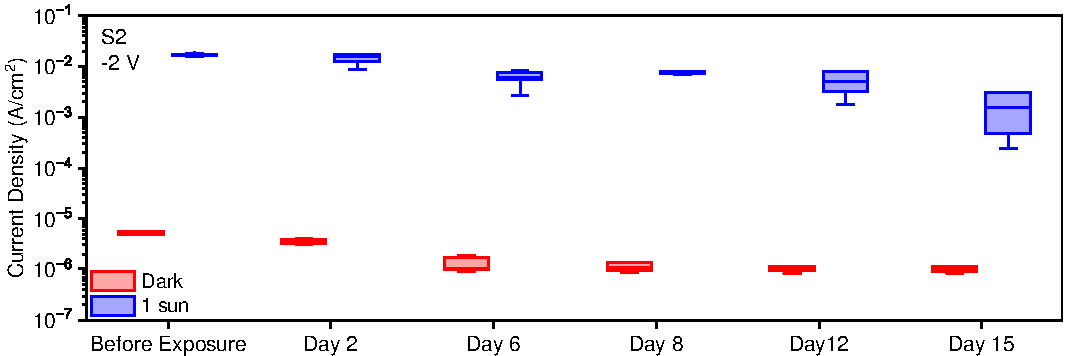
\includegraphics[width=\textwidth]{chapters/stability/imeges/AP44_2_Thesis.pdf} % Replace with your image file
        \caption*{(c)}
    \end{subfigure}
    \hfill
    \begin{subfigure}[t]{0.99\textwidth}
        \centering
        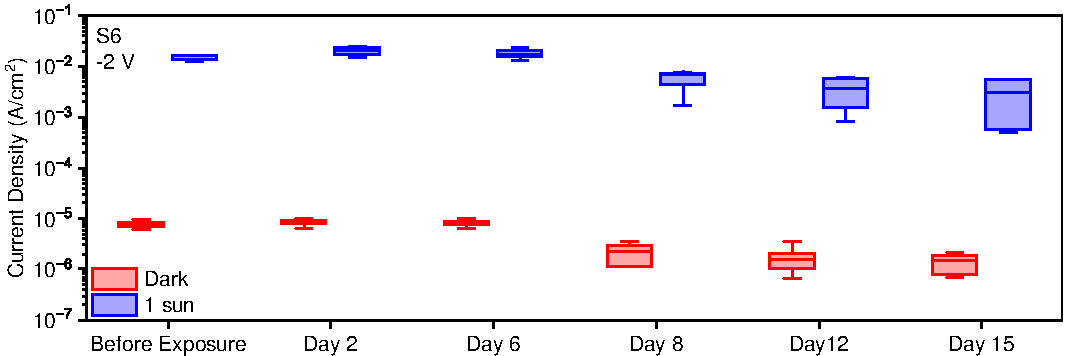
\includegraphics[width=\textwidth]{chapters/stability/imeges/AP44_4_Thesis.pdf} % Replace with your image file
        \caption*{(d)}
    \end{subfigure}
    \caption{Statistical results of current density at -2 V in dark and under 1-sun illumination for the top illuminated PePDs (a) S4, (b) S8, (c) S2, and (d) S6 (labeled according to the position of the substrate in Figure~\ref{fig:stability:ellipsometry:molar_ratio}b) as a function of exposure days to ambient conditions.}
    \label{fig:stability:pepd_stability}
\end{figure}


Building on the significant improvements in the ambient stability of \ch{CsPbI_2Br} films achieved through the combinatorial deposition approach, we proceed with the fabrication of top illuminated PePDs to evaluate the electrical performance of the stack upon exposure to the ambient atmosphere. The device architecture was the same as the one presented in Figure~\ref{fig:pix_pepd:cross_section_performance}a. In total, four samples were prepared, corresponding to positions S2, S4, S6, and S8 in Figure~\ref{fig:stability:ellipsometry:molar_ratio}b. In principle, samples S4 and S8 belong to the Pb-rich region and should convert within a few hours, while samples S2 and S6 belong to the Cs-rich region, and, when deposited on top of \ch{NiO_x}, can maintain their black phase stability for more than 26 days (Figure~\ref{fig:stability:no_rotation:300nm_ito_nio}). 

Prior to their exposure to ambient conditions, and despite the wide distribution of stoichiometries across their surface, all samples demonstrate high yield both in dark and under 1-sun illumination (Figure~\ref{fig:stability:pepd_stability}). Nevertheless, the samples in the Pb-rich region (S4 and S8) exhibit nearly half the photocurrent at -2 V compared to those in the Cs-rich region of the substrate holder (approx. 8 $mA/cm^2$ for the former and 17 $m A/cm^2$ for the latter). 

In terms of their ambient stability, and as expected, the perovskite in samples S4 and S8 converts almost instantaneously to the yellow phase, with their $J_{photo}$ dropping below 1 $mA/cm^2$ after one day of exposure in ambient conditions (Figure~\ref{fig:stability:pepd_stability}a and b, respectively). On the other hand, samples S2 and S6 maintain their initial performance for two and six days, respectively (Figure~\ref{fig:stability:pepd_stability}c and d). Even after 8 days in ambient conditions, their median $J_{photo}$ is above still 7 $mA/cm^2$. As time progresses, the median $J_{\text{photo}}$ decreases while the spread in device performance increases, indicating the ongoing conversion of the perovskite to the yellow phase. 

It is worth  highlighting that the stability of the bare films in the Cs-rich region of the substrate holder extended to at least 26 days, as it was shown in Figure~\ref{fig:stability:no_rotation:300nm_ito_nio}. Even after the repetition of the same deposition run (Figure~\ref{fig:appendix:stability_on_NiO_v2}), the sample in the position S2 maintained its black phase for at least 48 days. This indicates that the stability of the \ch{CsPbI_2Br} thin films is likely compromised when they are integrated in the complete device stack. It is plausible that the additional fabrication steps required for the deposition of the ETL and the ITO top contact generate processing conditions that have a negative impact on the ambient stability of the perovskite film. However, before drawing definitive conclusions, it is important to consider that the substrates used for the bare film stability study and the complete device stack are not identical. While both configurations terminate with a NiO layer, the bare films were deposited on glass/ITO, whereas the device stack was built on Si/TiN. This difference in substrate could significantly influence the growth of the \ch{NiO_x} layer, and by extension, the growth and properties of the perovskite layer itself.

Nevertheless, the improvement in ambient stability of the PePDs remains significant. Achieving devices that remain stable for over a week without any encapsulation opens up a new range of experiments and characterization methods that must be conducted under ambient conditions. The steps involved in dicing, bonding, and characterizing a perovskite-based imagers are examples of such processes.

\section{Conclusions}

In conclusion, this chapter critically evaluates the ambient stability of the black phase of \ch{CsPbI_2Br} thin films deposited via vacuum co-evaporation. While confirming prior research findings that CsBr-rich compositions exhibit superior ambient stability, a challenge in achieving consistent stoichiometry across multiple, in principle, identical depositions is identified. This variability hinders the reproducible fabrication of stable films and limits the comprehensive study of their properties. For this reason, a combinatorial deposition approach is adopted, enabled by the de-activation of substrate rotation during the co-evaporation process. This way, a continuous gradient of stoichiometries is deposited, mapped across the complete substrate holder by means of spectroscopic ellipsometry. Results indicate that the optimal CsBr:\ch{PbI_2} molar ratio for ambient stability lies between 1.15:1.00 and 1.35:1.00. Deviating beyond this range starts to compromise the stability of the deposited films. Additionally, preliminary results reveal that the stability is further enhanced by reducing the thickness of the perovskite layer or by depositing it on glass/ITO/\ch{NiO_x} substrates instead of bare glass ones. Leveraging these findings, top-illuminated perovskite photodetectors (PePDs) are fabricated. The best-performing devices maintained stable performance for eight days under ambient conditions, offering a promising path toward applications and characterization techniques that require occasional operation outside controlled environments. Future investigations should further explore whether the growth conditions imposed by the absence of substrate rotation have by themselves a positive impact on the films' ambient stability. 

%%%%%%%%%%%%%%%%%%%%%%%%%%%%%%%%%%%%%%%%%%%%%%%%%%
% Keep the following \cleardoublepage at the end of this file, 
% otherwise \includeonly includes empty pages.
\cleardoublepage

